\documentclass[11pt, a4paper]{article} % setsfont size and layout

%% required packages %%

\usepackage[margin=2.5cm]{geometry} % margins
\usepackage[english]{babel} % language (replace with german or ngerman for german texts)
\usepackage[utf8]{inputenc} % Umlaute
\usepackage{amsmath}		% math formulas
\usepackage{graphicx}		% graphics
\usepackage{fancyhdr}		% header and footer on every page
\usepackage{setspace}		% line space (e.g. \singlespacing, \onehalfspacing or \doublespacing)
\usepackage{xcolor}
\usepackage{pdflscape}
\usepackage{rotating}
\usepackage[boxruled, lined, vlined]{algorithm2e}
\SetKwFor{For}{for (}{) $\lbrace$}{$\rbrace$}
\usepackage{bm}
\usepackage{caption}
\usepackage{subcaption}
\usepackage{float}
\usepackage{multicol}

\begin{document}
	
%% Some more settings %%
	
\setlength{\parindent}{0pt} % first line in paragraph will not be indented
\onehalfspacing				% 1.5 line spacing
%\thispagestyle{empty}		% no header and page number on first page


%% Header on first page with course information etc. %%
\begin{tabular}{p{15.5cm}}
	{\large \textbf{Inrobin}} \\
	Gareth W. Peters  \\ 
	Dorota Toczydłowska\\
	Marta Campi\\
	\hline
	\\
\end{tabular}

\vspace*{0.3cm}				% vertical space between header on top of the page and main heading


\begin{center}
	{\LARGE \textbf{Experiment two:}}
	\vspace{2mm}	
\end{center} 

\section*{Detecting Spectral Content}
Set the notation of this experiment as follows:

$\Omega$ is the set of $M_{true}$ vectors of parameters where each vector is $J$ dimensional \\
$\Omega = \Big\{ \Psi^1, \ldots, \Psi^{M_{true}} \Big\}$\\
Let $\Psi^{j} = [\Psi^{j}_1, \ldots, \Psi^{j}_J]$ which is the $j$th element of $\Omega$ set\\
$\Psi^j_h$ is $h$th element of $\Psi^{j}$\\
$k(\cdot, \cdot;\Psi)$ a kernel function from parameterized by the parameter $\Psi$,  $k: \mathcal{R} \times \mathcal{R} \rightarrow \mathcal{R}$\\ 
Let $\mathbf{t}$ be a $1\times N$ vector of real numbers\\
$\mathbf{K} = k(\mathbf{t}, \mathbf{t};\Psi = \Psi)$\\
$j \in \Big\{ 1, \cdots, M_{true} \Big\}$, $m \in \Big\{ 1, \cdots, M \Big\}$, $h \in \Big\{1, \ldots, J \Big\}$\\ %maybe change notation
$n_{j,m}$ number of IMFs

\hfill

\begin{algorithm}[H]


\label{algo_exp1}
\caption{Algorithm}

\BlankLine
\addtolength\linewidth{-12ex}

\KwIn{Define $k, J, \Omega, \mathbf{t}, M_{true}$\\
Set $m,j, J$}
%\KwOut{CKTA between $\mathbf{S}_{N \times N}^{(m)}$ and Kernel Gram Matrix $\mathbf{K}_{(test,i)}$ }

\begin{enumerate}

\item Evaluate each Gram Matrix $\mathbf{K}^{(j)}_h = k(\mathbf{t},\mathbf{t}; \Psi^{(j)}_h)$ parametrized by the $j$th parameter from $\Omega$. There are $J$ Gram Matrices since $h = 1, \dots, J$ \\

\item Simulate $\mathbf{y}_{j,h}^{(m)} \sim \mathcal{N}(0, \mathbf{K}^{(j)}_h)$ an N dimensional vector for each Gram Matrix $\mathbf{K}^{(j)}_h$, therefore we have $J$ one dimensional vectors of length $N$.\\

\item Compute $ \mathbf{x}^{(m)}_j = \sum_{h=1}^{J} \mathbf{y}_{j,h}^{(m)} $

\item Fit a spline through each $\mathbf{x}_j^{(m)}$ denoted as $\hat{\mathbf{x}}_j^{(m)}$.

\item Apply the EMD to $ \hat{\mathbf{x}}_j^{(m)}$ to get the IMFs decomposition and collect all the IMFs generated up to the stopping criterion chosen denoted as $\bm{\gamma}^{(m)}_{j,1}, \bm{\gamma}_{j,2}^{(m)}, \dots, \bm{\gamma}_{j,v_{j,m}}^{(m)}$. For each $j$ and for each $m$ we might have different number of IMFs denote by $v_{j,m}$.

\item Compute the Instantaneous Frequency of each IMF denoted as $\bm{f}^{(m)}_{j,1}, \bm{f}_{j,2}^{(m)}, \dots, \bm{f}_{j,v_{j,m}}^{(m)}$.
\item Compare the frequencies with Spectral Component of the kernels


\end{enumerate}

\end{algorithm}


\hfill

\newpage




\begin{algorithm}[H]


\label{algo_exp1}
\caption{Algorithm}

\BlankLine
\addtolength\linewidth{-12ex}

\KwIn{Define $k, J, \Omega, \mathbf{t}, M_{true}$}

\For{$m = 1:M$}{

\For{$h = 1:J$}{
Evaluate each Gram Matrix $\mathbf{K}^{(j)}_h = k(\mathbf{t},\mathbf{t}; \Psi^{(j)}_h)$ parametrized by the $j$th parameter from $\Omega$. There are $J$ Gram Matrices since $h = 1, \dots, J$ \\

Simulate $\mathbf{y}_{j,h}^{(m)} \sim \mathcal{N}(0, \mathbf{K}^{(j)}_h)$ an N dimensional vector for each Gram Matrix $\mathbf{K}^{(j)}_h$, therefore we have $J$ one dimensional vectors of length $N$.\\

Compute $ \mathbf{x}^{(m)}_j = \sum_{h=1}^{J} \mathbf{y}_{j,h}^{(m)} $\\
}

Fit a spline through each $\mathbf{x}_j^{(m)}$ denoted as $\hat{\mathbf{x}}_j^{(m)}$.\\

Apply the EMD to $ \hat{\mathbf{x}}_j^{(m)}$ to get the IMFs decomposition and collect all the IMFs generated up to the stopping criterion chosen denoted as $\bm{\gamma}^{(m)}_{j,1}, \bm{\gamma}_{j,2}^{(m)}, \dots, \bm{\gamma}_{j,v_{j,m}}^{(m)}$. For each $j$ and for each $m$ we might have different number of IMFs denote by $v_{j,m}$.\\

Compute the Instantaneous Frequency of each IMF denoted as $\bm{f}^{(m)}_{j,1}, \bm{f}_{j,2}^{(m)}, \dots, \bm{f}_{j,v_{j,m}}^{(m)}$. \\

Compare the frequencies with Spectral Component of the kernels
}

\end{algorithm}


\hfill


Example:
Periodic Kernel: $\Omega = \left\lbrace (l_1,p_1), (l_1,p_2), (l_1,p_3), (l_2,p_1), (l_2,p_2), (l_2,p_3)  \right\rbrace$, $j = 2$, $h = 1:6$, $J = 6$,
$\Psi^{j} = [\Psi^{j}_1, \dots , \Psi^{j}_6]$ and $\Psi^j_1 = \left\lbrace  l_1, p_1 \right\rbrace$, $\dots$, $\Psi^j_6 = \left\lbrace  l_2, p_3 \right\rbrace$.\\ 

\textbf{Stopping Criteria for the sifting procedure}
\small

\begin{itemize}
\item \textbf{Cauchy-Type Convergence (SD)}.
\cite{Huang1998} proposed such criterion to limit amplitude and frequency modulations through a certain threshold of the standard deviation of two consecutive sifting results.

\scriptsize
\begin{equation}
SD = \sum_{t=0}^{T}\left[ \frac{|\left(h_{1\left(k-1\right)}\left(t\right)-h_{1k}\left(t\right)\right)|^2}{h_{1\left(k-1\right)}^2 \left(t\right)} \right]
\end{equation}

\small

\item \textbf{Mean Fluctuations Threshold}. 
\cite{Rilling2003} proposed three different thresholds allowing for small fluctuations of the mean and locally large excursions. The thresholds are $\alpha$, $\theta_1$ and $\theta_2$. For $\left(1-\alpha\right)$ data, the criterion keeps sifting if $\sigma\left(t\right) < \theta_1$, while for the remaining fraction if $\sigma\left(t\right) < \theta_2$. The quantities are defines as:

\scriptsize
\begin{multicols}{3}
\begin{equation*}
\sigma\left(t\right):= \Bigl| \frac{m\left(t\right)}{a\left(t\right)} \Bigr|
\end{equation*}

\begin{equation*}
a\left(t\right):= \frac{S(e_1^S)-S(e_2^S)}{2}
\end{equation*}

\begin{equation*}
m\left(t\right):= \frac{S(e_1^S)+S(e_2^S)}{2}
\end{equation*}
\end{multicols}{3}

\small

\item \textbf{Energy Difference Tracking}.
The assumption of this criterion is that the EMD provides IMFs and a residual mutually orthogonal. If $c_1$ is extracted from the signal, the sum of its energy and those of the residual signal ($E_{tot}$) is equal to the energy of the original signal ($E_S$ ). If not, there must be a difference called energy error ($E_{err}$). The sifting procedure stops when both $E_{err}$ and the mean value are small enough. $E_{err}$ for $c_1$ is defined as:
\scriptsize
\begin{equation}
E_{err} = E_{tot} - E_S = \int c_1^2(t) dt - \int S(t) c_1(t)dt
\end{equation}
\small

\item \textbf{Orthogonality Criterion}.
\cite{LinLin} underline the fact that any IMF, in this case $c_1$ should satisfy:
\scriptsize
\begin{equation}
\sum_{t=1}^N c_1\left(t\right)\left(x\left(t\right) - c_1 \left(t\right)\right) = 0
\end{equation}
\small
which states the orthogonality of the IMFs. They determine the following index and the sifting procedure stops once that it reaches a certain minimum value:
\scriptsize
\begin{equation}
OC = \left|\sum_{t=1}^N \frac{m\left(t\right) S(t)}{m\left(t\right)\left(S(t) - m\left(t\right) \right)} \right| \quad \mbox{where} \quad m\left(t\right) = \frac{S(e_1^S)+S(e_2^S)}{2}
\end{equation}
\end{itemize}

\normalsize
\begin{figure}[H]
\begin{subfigure}{.5\textwidth}
  \centering
  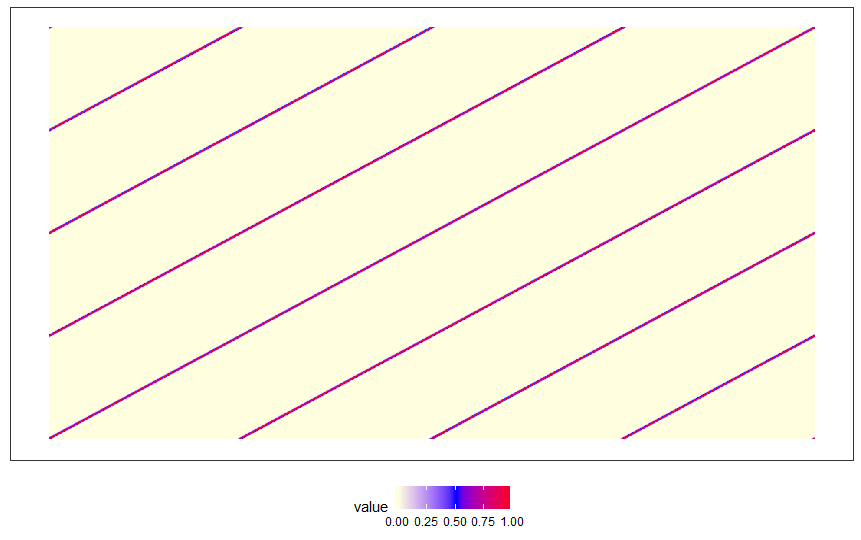
\includegraphics[width=.8\linewidth]{KSE_N1000_l005_p025.png}
  \label{fig:sfig1}
\end{subfigure}%
\begin{subfigure}{.5\textwidth}
  \centering
  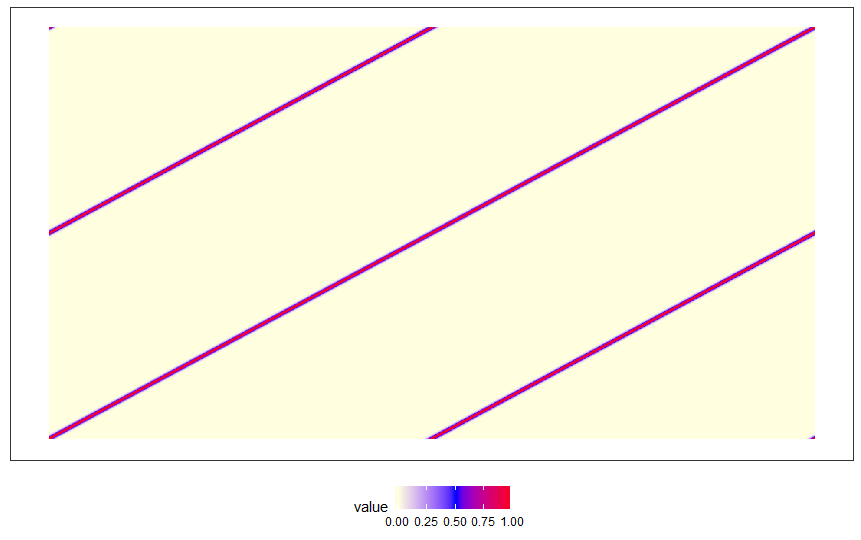
\includegraphics[width=.8\linewidth]{KSE_N1000_l0005_p05.png}
  \label{fig:sfig2}
\end{subfigure}\\
\begin{subfigure}{.5\textwidth}
  \centering
  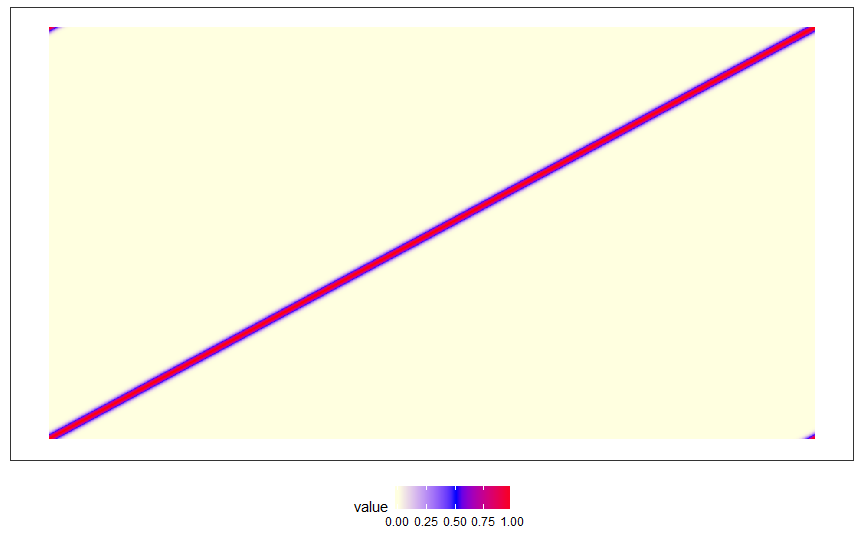
\includegraphics[width=.8\linewidth]{KSE_N1000_l005_p1.png}
  \label{fig:sfig2}
\end{subfigure}
\caption{Heatmaps of Gram Matrices for the periodic Kernel with $N = 1000, l = 0.05, p = 0.25, 0.5, 1 $}
\label{fig:fig}
\end{figure}

\begin{figure}[H]
\begin{subfigure}{.5\textwidth}
  \centering
  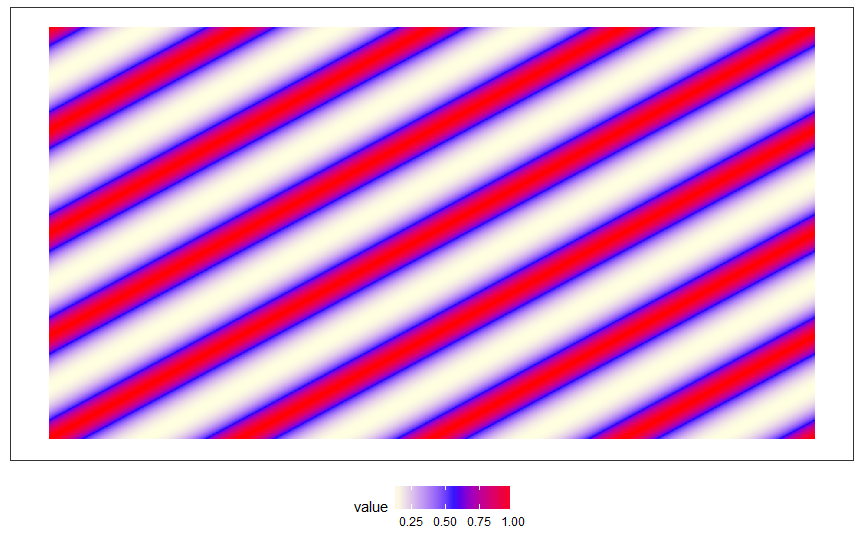
\includegraphics[width=.8\linewidth]{KSE_N1000_l1_p025.png}
  \label{fig:sfig1}
\end{subfigure}%
\begin{subfigure}{.5\textwidth}
  \centering
  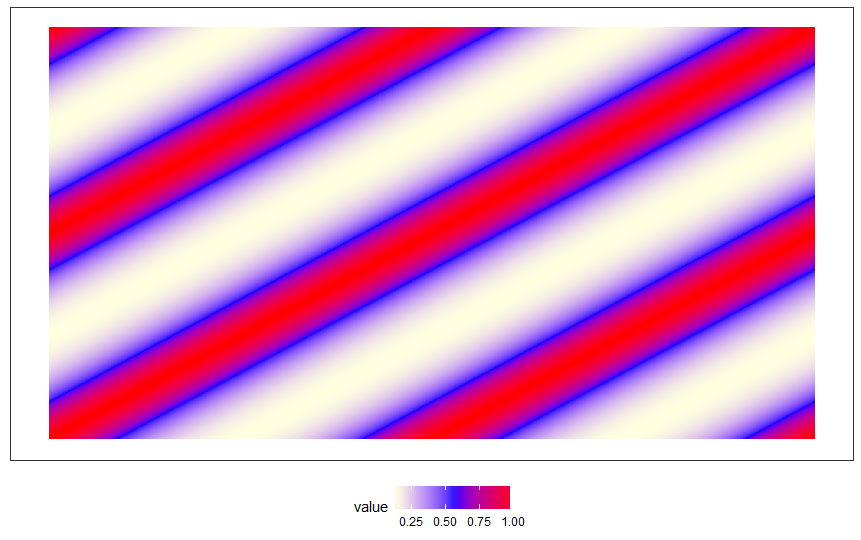
\includegraphics[width=.8\linewidth]{KSE_N1000_l1_p05.png}
  \label{fig:sfig2}
\end{subfigure}\\
\begin{subfigure}{.5\textwidth}
  \centering
  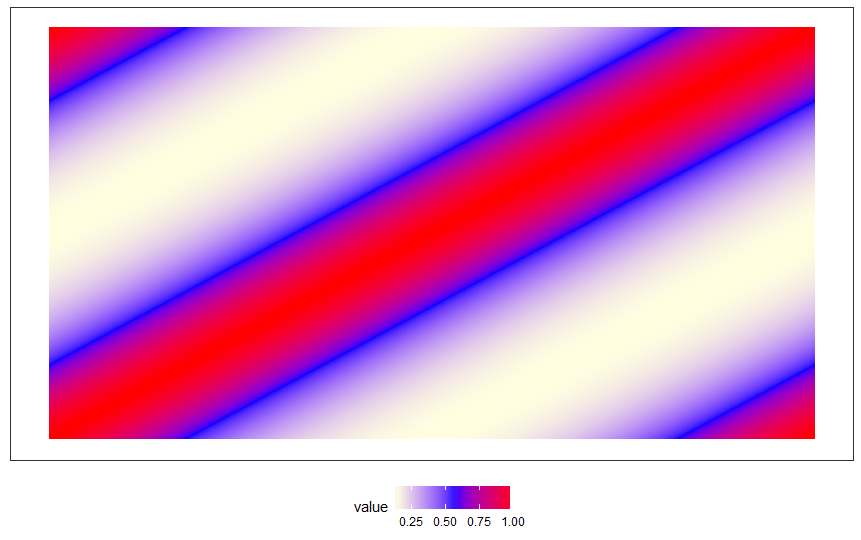
\includegraphics[width=.8\linewidth]{KSE_N1000_l1_p1.png}
  \label{fig:sfig2}
\end{subfigure}
\caption{Heatmaps of Gram Matrices for the periodic Kernel with $N = 1000, l = 1, p = 0.25, 0.5, 1$}
\label{fig:fig}
\end{figure}



\newgeometry{left=2.3cm,bottom=0.1cm} 

\begin{figure}[H]
\begin{subfigure}{1.1\textwidth}
  \centering
  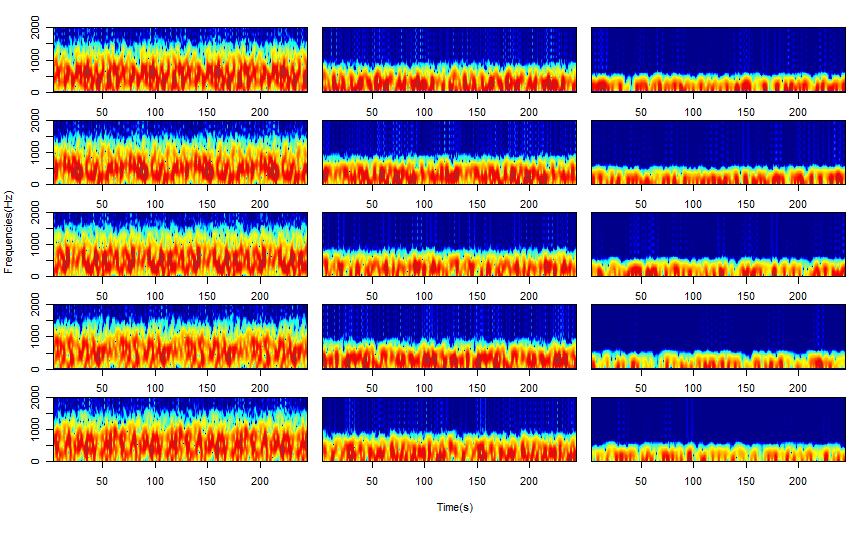
\includegraphics[width=\linewidth]{spectro_N1000_l005_ym_1_5.png}
  \label{fig:sfig1}
\end{subfigure}\\
\begin{subfigure}{1.1\textwidth}
  \centering
  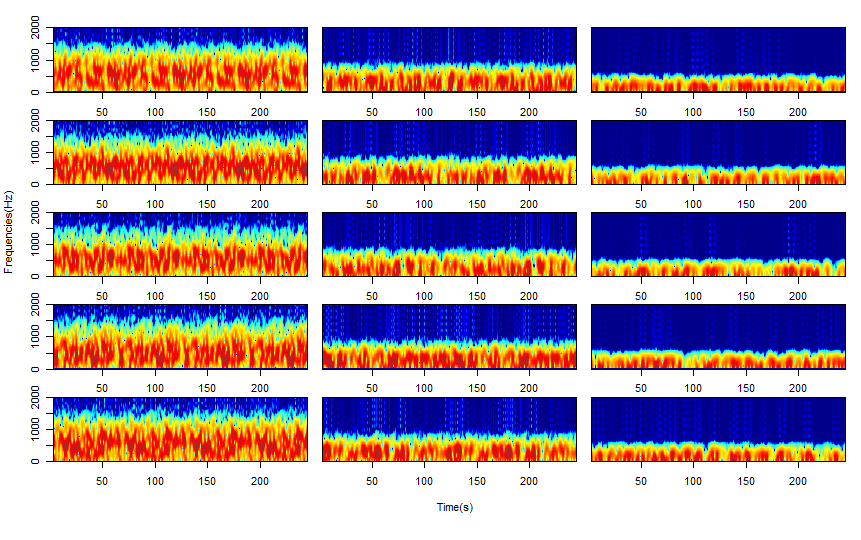
\includegraphics[width=\linewidth]{spectro_N1000_l005_ym_6_10.png}
  \label{fig:sfig2}
\end{subfigure}
\caption{$N = 1000, l = 0.05$. Spectrograms of the $ y^{(m)}$ constructed with the above matrices for $m = 1, \dots, 10$.  }
\label{fig:fig}
\end{figure}

\restoregeometry



\newgeometry{left=2.3cm,bottom=0.1cm} 

\begin{figure}[H]
\begin{subfigure}{1.1\textwidth}
  \centering
  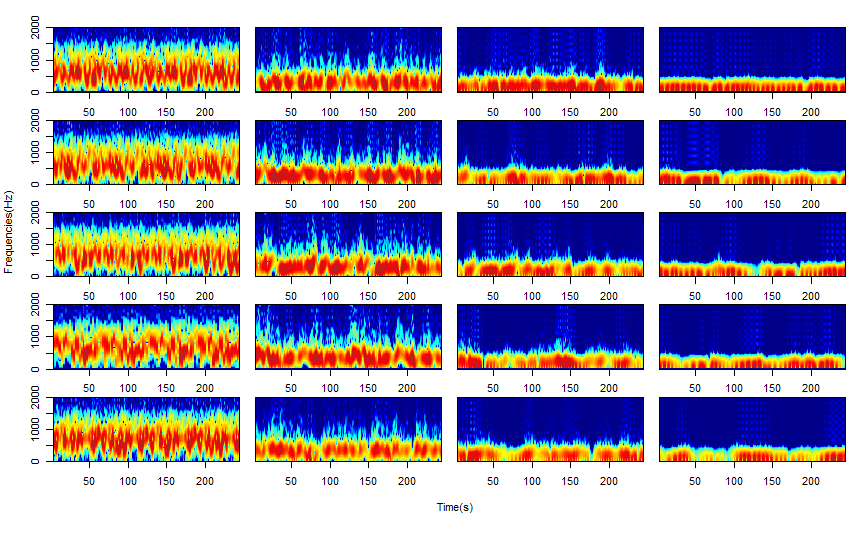
\includegraphics[width=\linewidth]{spectro_N1000_l005_IMF_1_5.png}
  \label{fig:sfig1}
\end{subfigure}\\
\begin{subfigure}{1.1\textwidth}
  \centering
  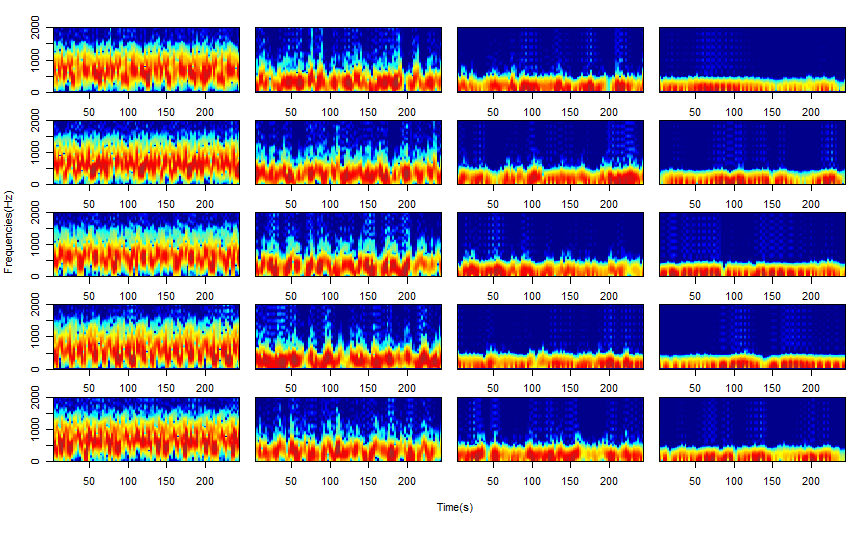
\includegraphics[width=\linewidth]{spectro_N1000_l005_IMF_6_10.png}
  \label{fig:sfig2}
\end{subfigure}
\caption{$N = 1000, l = 0.05, p = 0.25, 0.5, 1$. Spectrograms of the IMFs extracted by $\hat{x}^{(m)}$ constructed with the above $y_m$ for $m = 1, \dots, 10$.}
\label{fig:fig}
\end{figure}
\restoregeometry



\newgeometry{left=2.3cm,bottom=0.1cm} 

\begin{figure}[H]
\begin{subfigure}{1.1\textwidth}
  \centering
  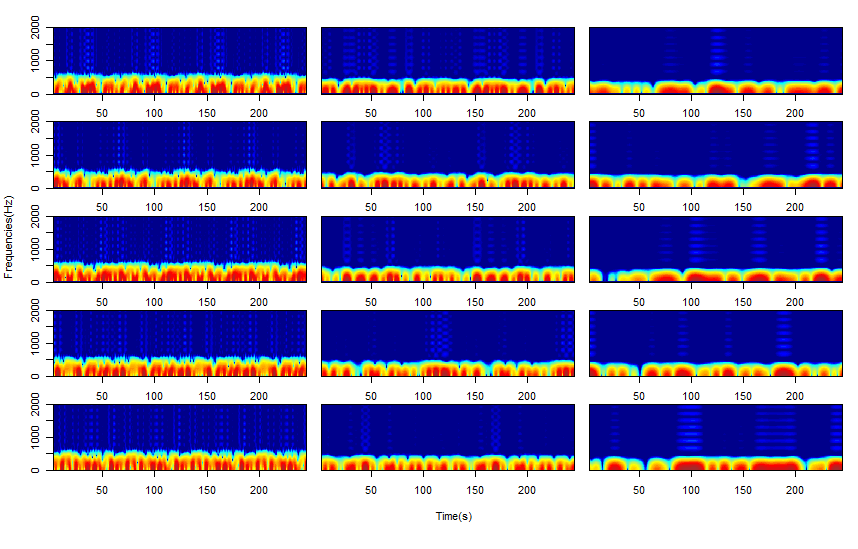
\includegraphics[width=\linewidth]{spectro_N1000_l020_y_m_1_5.png}
  \label{fig:sfig1}
\end{subfigure}\\
\begin{subfigure}{1.1\textwidth}
  \centering
  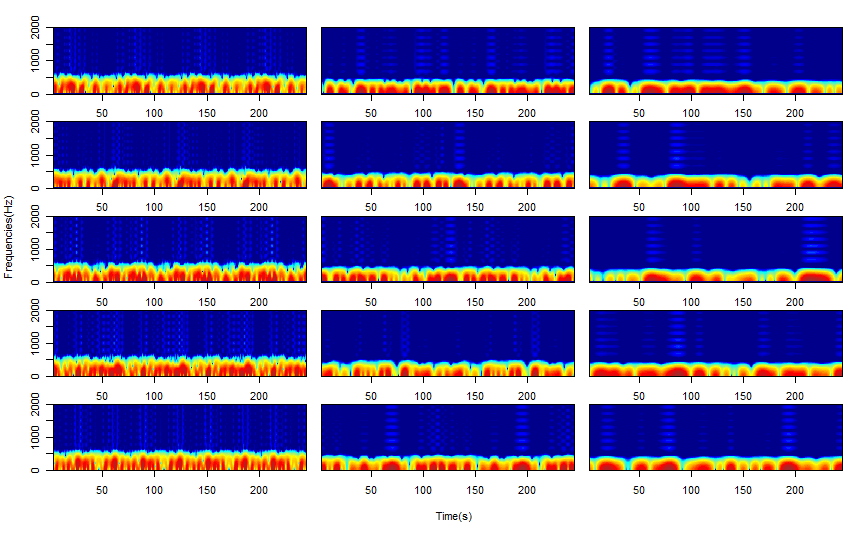
\includegraphics[width=\linewidth]{spectro_N1000_l020_y_m_6_10.png}
  \label{fig:sfig2}
\end{subfigure}
\caption{$N = 1000, l = 0.2, p = 0.25, 0.5, 1$. Spectrograms of the $y^{(m)}$ components constructed with the above matrices for $m = 1, \dots, 10$.  }
\label{fig:fig}
\end{figure}

\restoregeometry



\newgeometry{left=2.3cm,bottom=0.1cm} 

\begin{figure}[H]
\begin{subfigure}{1.1\textwidth}
  \centering
  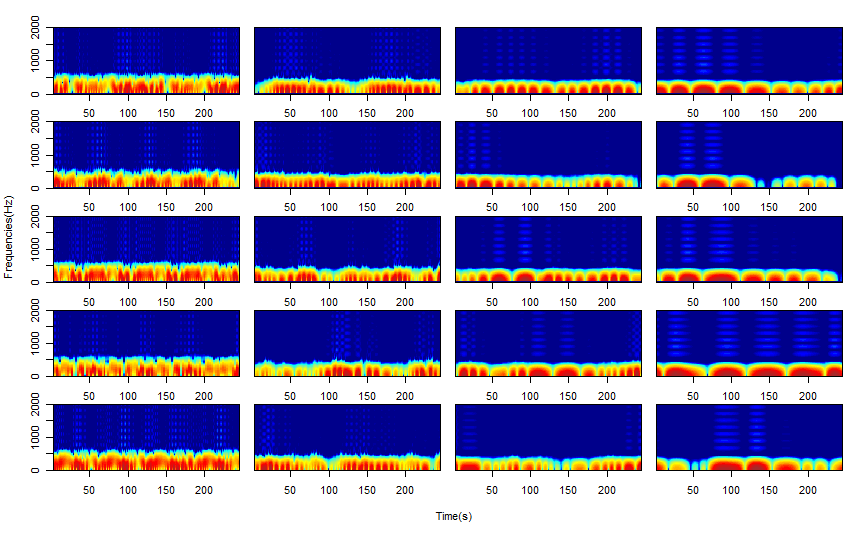
\includegraphics[width=\linewidth]{spectro_N1000_l020_IMF_1_5.png}
  \label{fig:sfig1}
\end{subfigure}\\
\begin{subfigure}{1.1\textwidth}
  \centering
  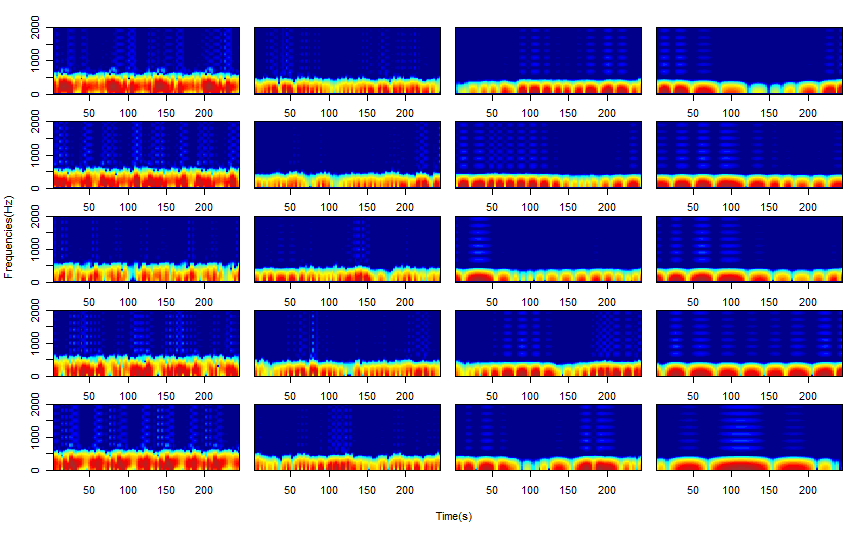
\includegraphics[width=\linewidth]{spectro_N1000_l020_IMF_6_10.png}
  \label{fig:sfig2}
\end{subfigure}
\caption{$N = 1000, l = 0.2, p = 0.25, 0.5, 1$. Spectrograms of the IMFs extracted by $\hat{x}^{(m)}$ constructed with the above $y^{(m)}$ for $m = 1, \dots, 10$.}
\label{fig:fig}
\end{figure}
\restoregeometry


\newgeometry{left=2.3cm,bottom=0.1cm} 

\begin{figure}[H]
\begin{subfigure}{1.1\textwidth}
  \centering
  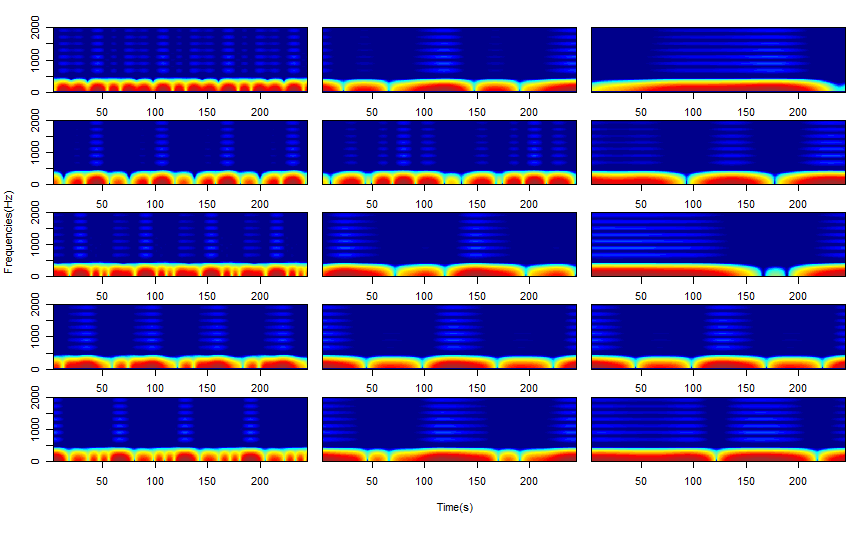
\includegraphics[width=\linewidth]{spectro_N1000_l1_y_m_1_5.png}
  \label{fig:sfig1}
\end{subfigure}\\
\begin{subfigure}{1.1\textwidth}
  \centering
  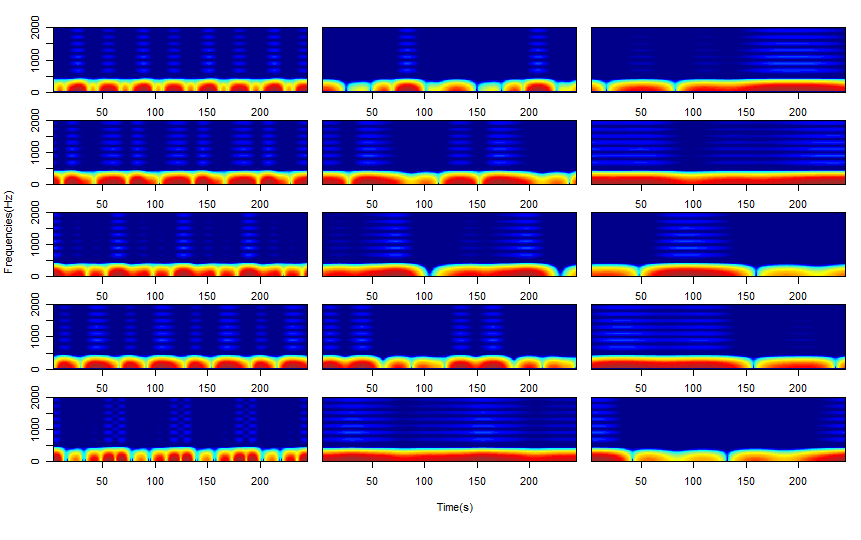
\includegraphics[width=\linewidth]{spectro_N1000_l1_y_m_6_10.png}
  \label{fig:sfig2}
\end{subfigure}
\caption{$N = 1000, l = 1, p = 0.25, 0.5, 1$. Spectrograms of the $ y^{(m)}$ components constructed with the above matrices for $m = 1, \dots, 10$  }
\label{fig:fig}
\end{figure}
\restoregeometry


\newgeometry{left=2.3cm,bottom=0.1cm} 

\begin{figure}[H]
\begin{subfigure}{1.1\textwidth}
  \centering
  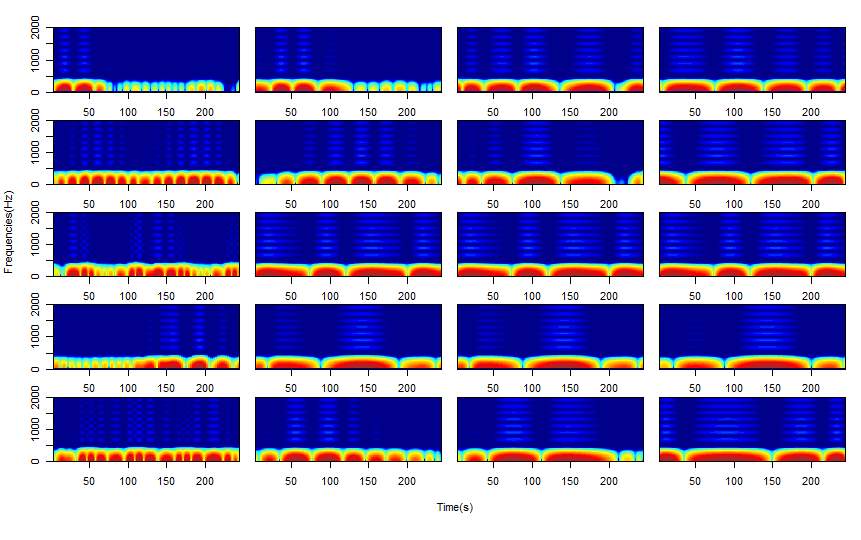
\includegraphics[width=\linewidth]{spectro_N1000_l1_IMF_1_5.png}
  \label{fig:sfig1}
\end{subfigure}\\
\begin{subfigure}{1.1\textwidth}
  \centering
  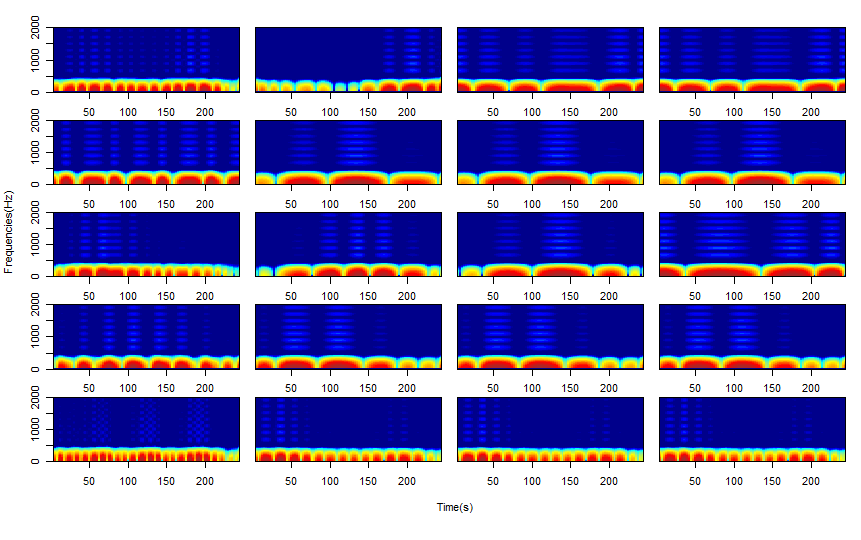
\includegraphics[width=\linewidth]{spectro_N1000_l1_IMF_6_10.png}
  \label{fig:sfig2}
\end{subfigure}
\caption{$N = 1000, l = 1, p = 0.25, 0.5, 1$, $m = 1, \dots = 10$. Spectrograms of the IMFs extracted by $\hat{x}^{(m)}$ constructed with the above $y^{(m)}$.}
\label{fig:fig}
\end{figure}
\restoregeometry



\newgeometry{left=2.3cm,bottom=0.1cm} 

\begin{figure}
\begin{subfigure}{1.1\textwidth}
  \centering
  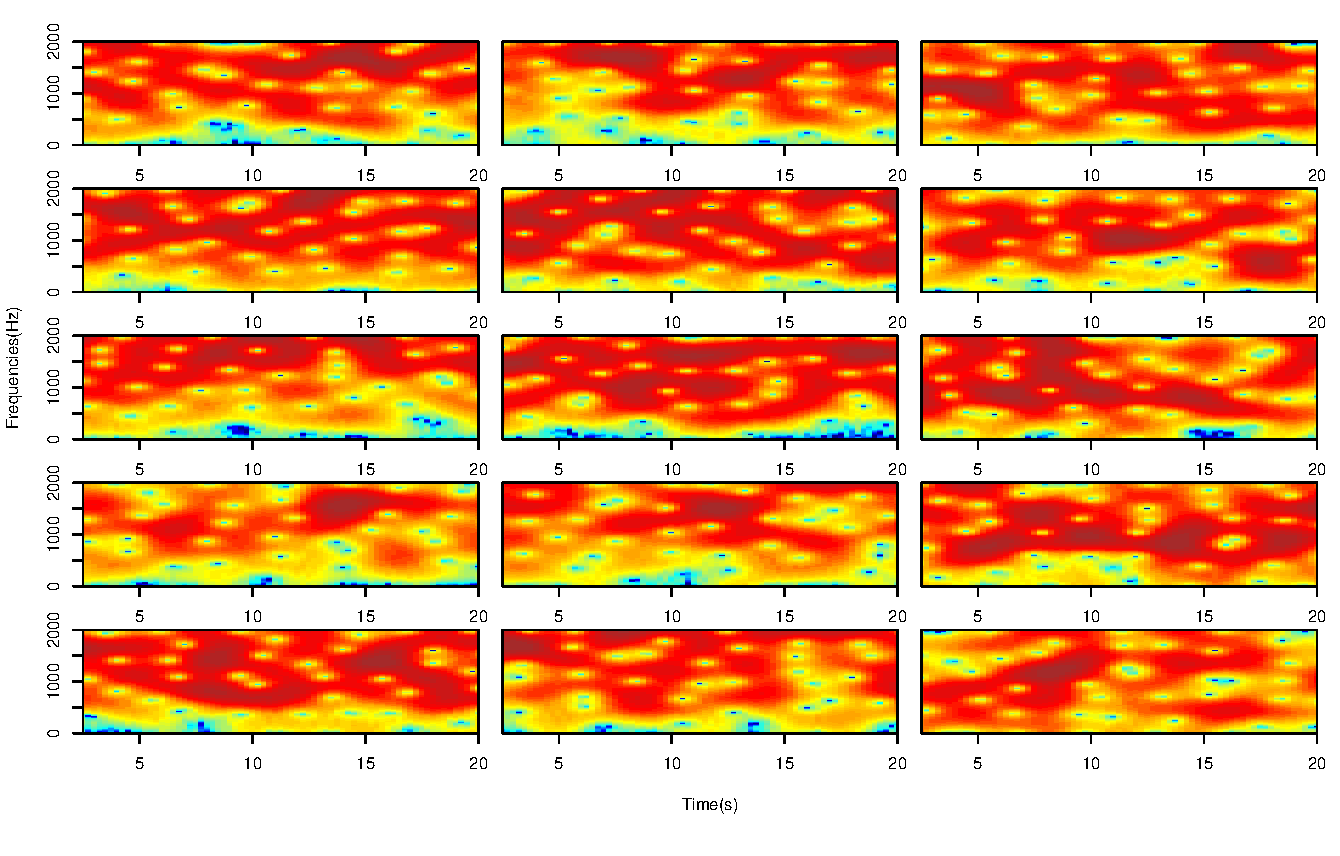
\includegraphics[width=\linewidth]{spectro_N100_l005_y_m_1_5.pdf}
%  \caption{1a}
  \label{fig:sfig1}
\end{subfigure}\\
\begin{subfigure}{1.1\textwidth}
  \centering
  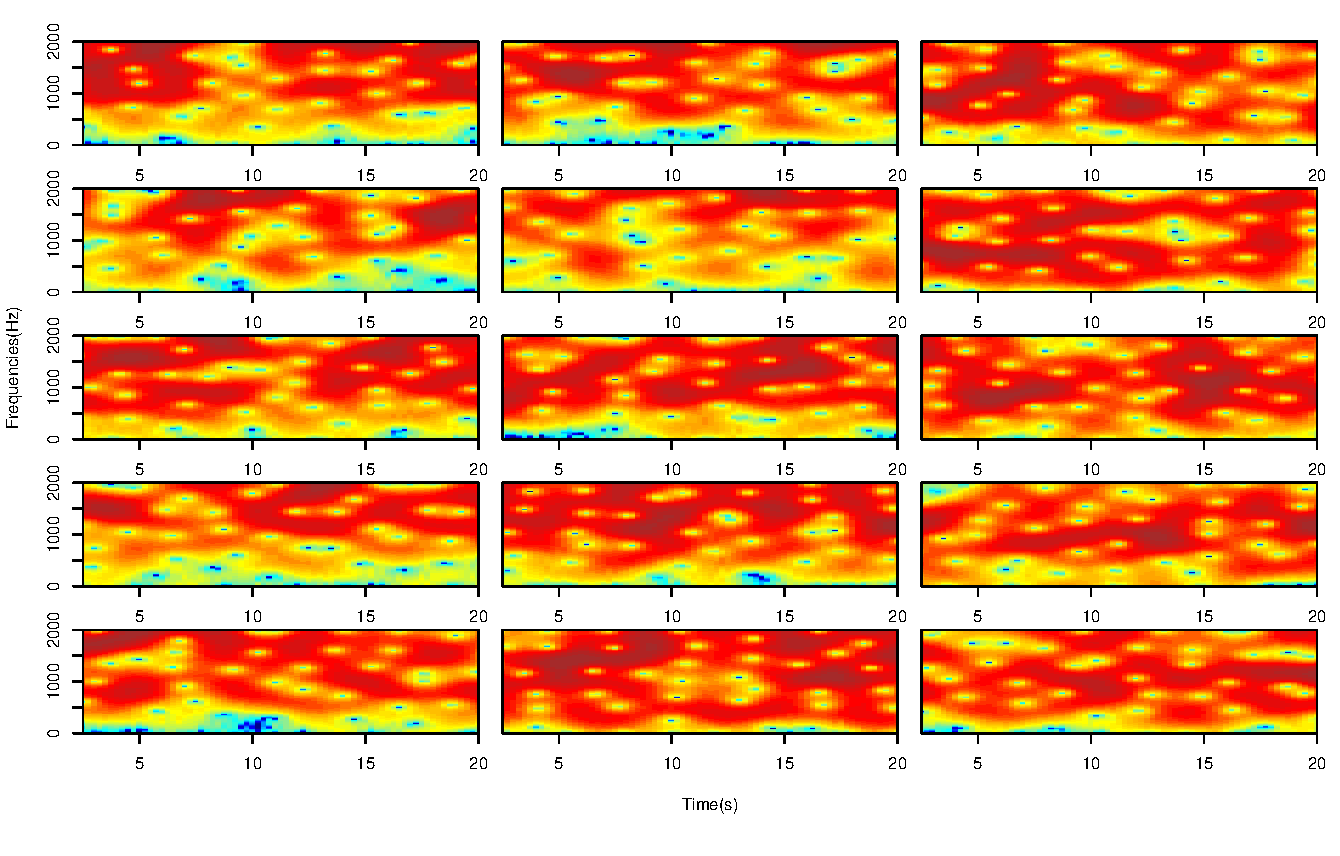
\includegraphics[width=\linewidth]{spectro_N100_l005_y_m_6_10.pdf}
%  \caption{1b}
  \label{fig:sfig2}
\end{subfigure}
\label{fig1}
\caption{$N = 100$, $l = 0.05$, $p = 0.25, 0.5, 1.00$. Spectrograms of the $y^{(m)}$ components.}
\end{figure}

\restoregeometry


\newgeometry{left=2.3cm,bottom=0.1cm} 

\begin{figure}
\begin{subfigure}{1.1\textwidth}
  \centering
  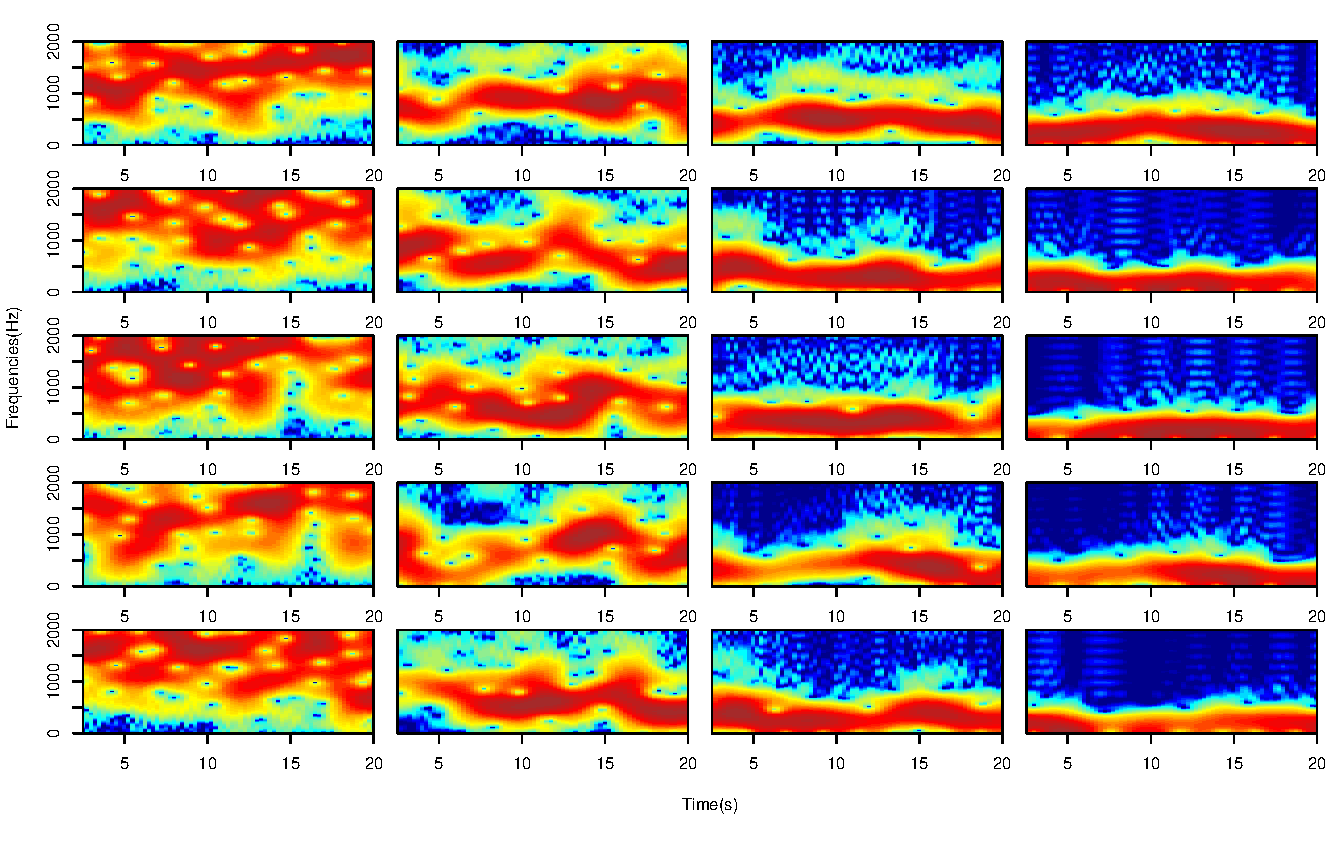
\includegraphics[width=\linewidth]{spectro_N100_l005_IMF_m_1_5.pdf}
%  \caption{1a}
  \label{fig:sfig1}
\end{subfigure}\\
\begin{subfigure}{1.1\textwidth}
  \centering
  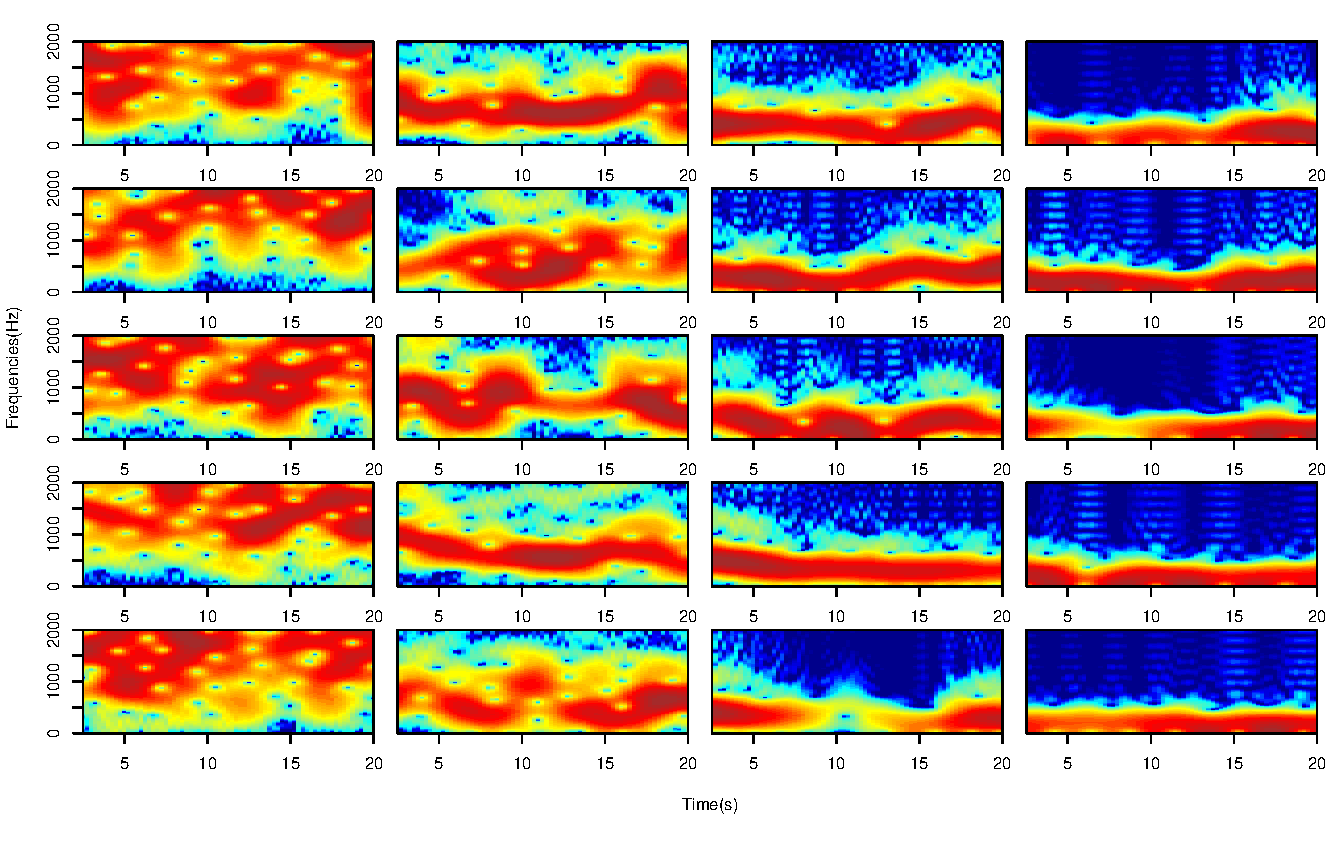
\includegraphics[width=\linewidth]{spectro_N100_l005_IMF_m_6_10.pdf}
%  \caption{1b}
  \label{fig:sfig2}
\end{subfigure}
\label{fig1}
\caption{$N = 100$, $l = 0.05$, $p = 0.25, 0.5, 1.00$. Spectrograms of the IMFs extracted by $\hat{x}^{(m)}$.}
\end{figure}

\restoregeometry




\newgeometry{left=2.3cm,bottom=0.1cm} 

\begin{figure}
\begin{subfigure}{1.1\textwidth}
  \centering
  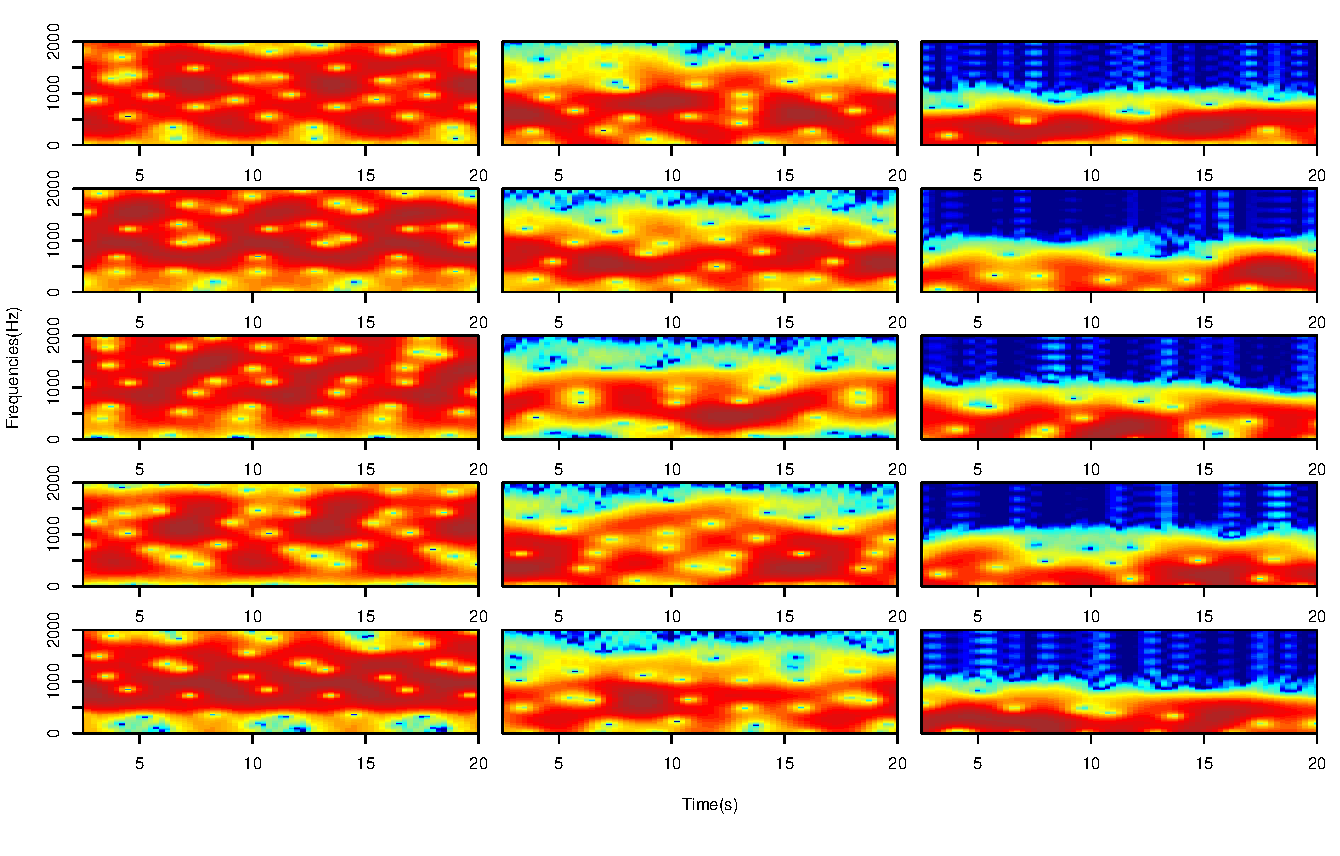
\includegraphics[width=\linewidth]{spectro_N100_l020_y_m_1_5.pdf}
%  \caption{1a}
  \label{fig:sfig1}
\end{subfigure}\\
\begin{subfigure}{1.1\textwidth}
  \centering
  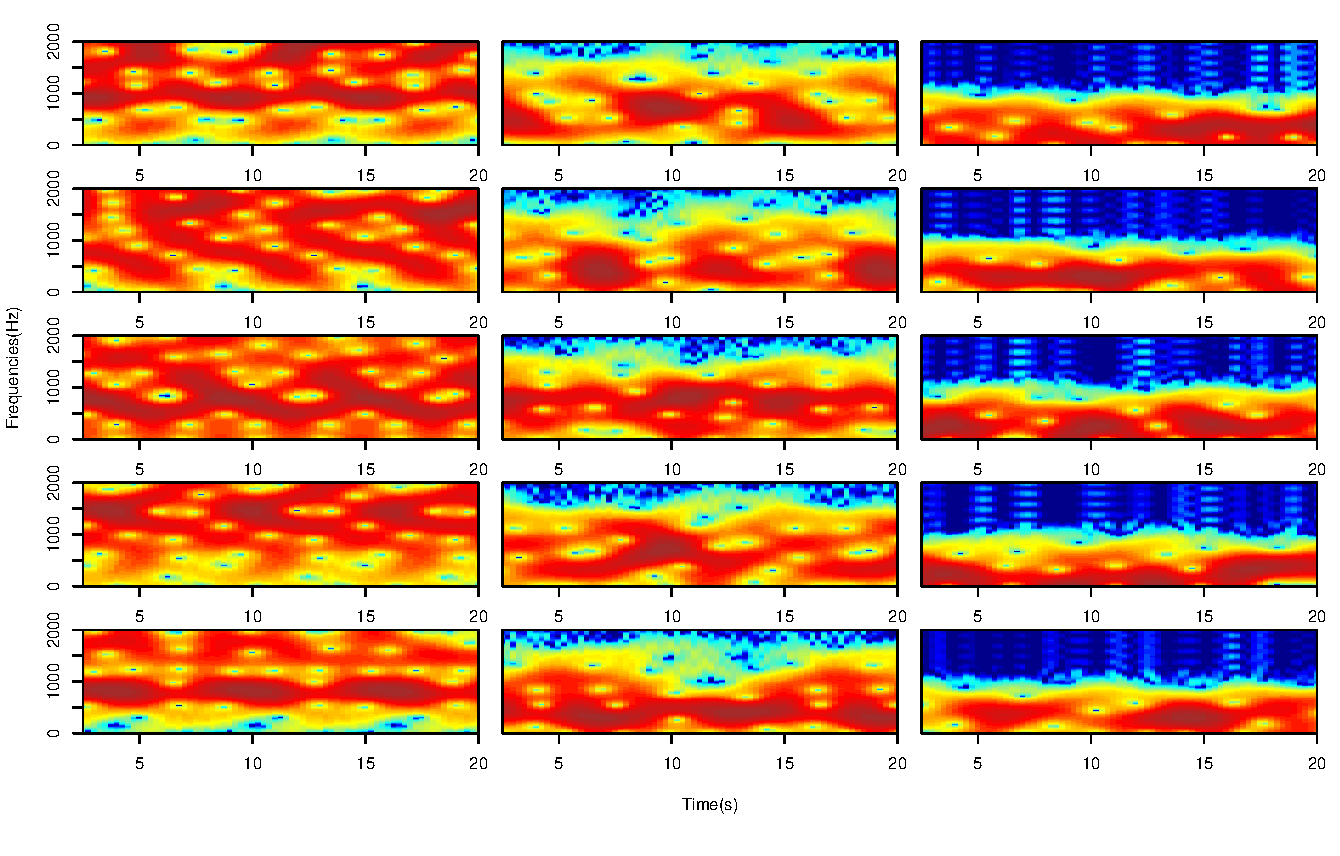
\includegraphics[width=\linewidth]{spectro_N100_l020_y_m_6_10.pdf}
%  \caption{1b}
  \label{fig:sfig2}
\end{subfigure}
\label{fig1}
\caption{$N = 100$, $l = 0.2$, $p = 0.25, 0.5, 1.00$. Spectrograms of the $y^{(m)}$ components.}
\end{figure}

\restoregeometry


\newgeometry{left=2.3cm,bottom=0.1cm} 

\begin{figure}
\begin{subfigure}{1.1\textwidth}
  \centering
  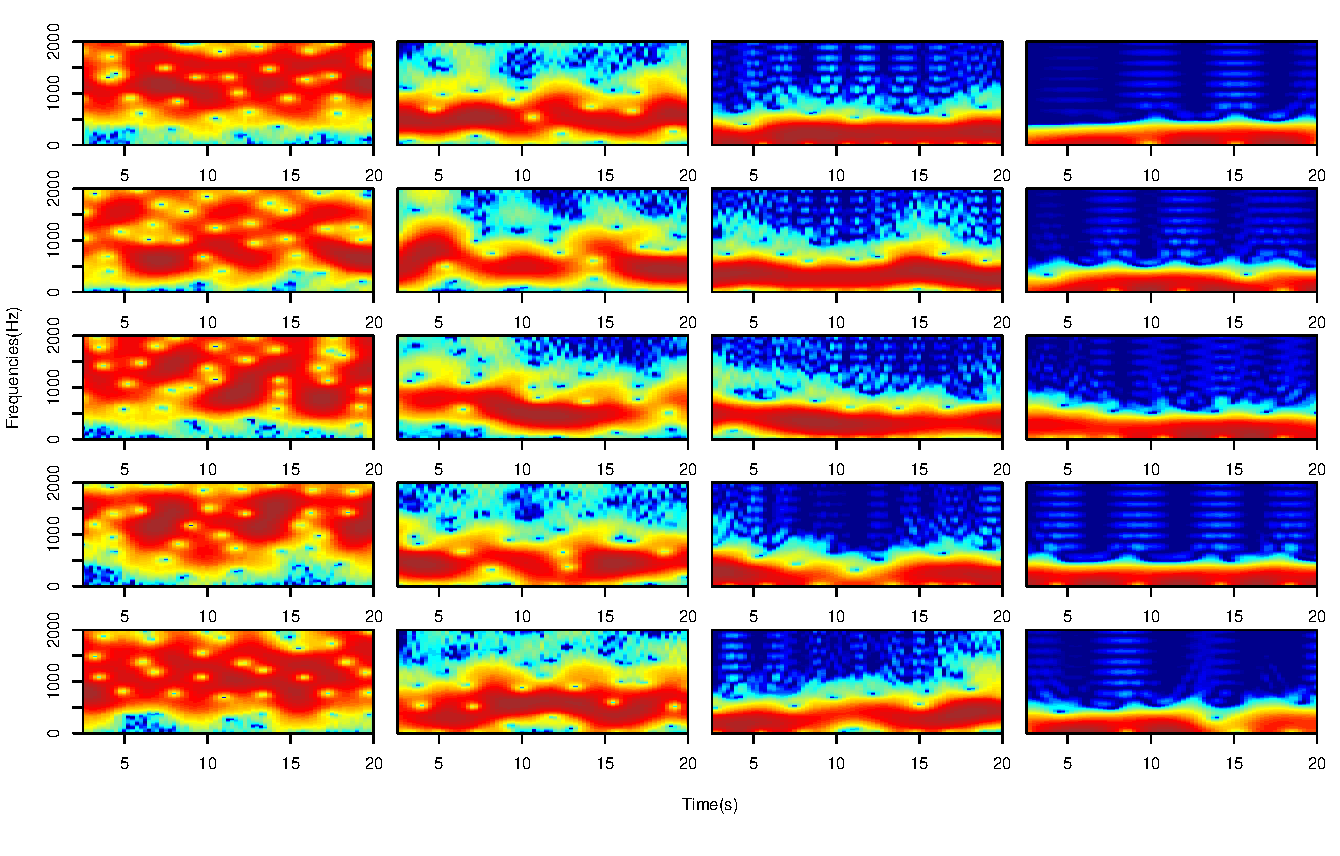
\includegraphics[width=\linewidth]{spectro_N100_l020_IMF_1_5.pdf}
%  \caption{1a}
  \label{fig:sfig1}
\end{subfigure}\\
\begin{subfigure}{1.1\textwidth}
  \centering
  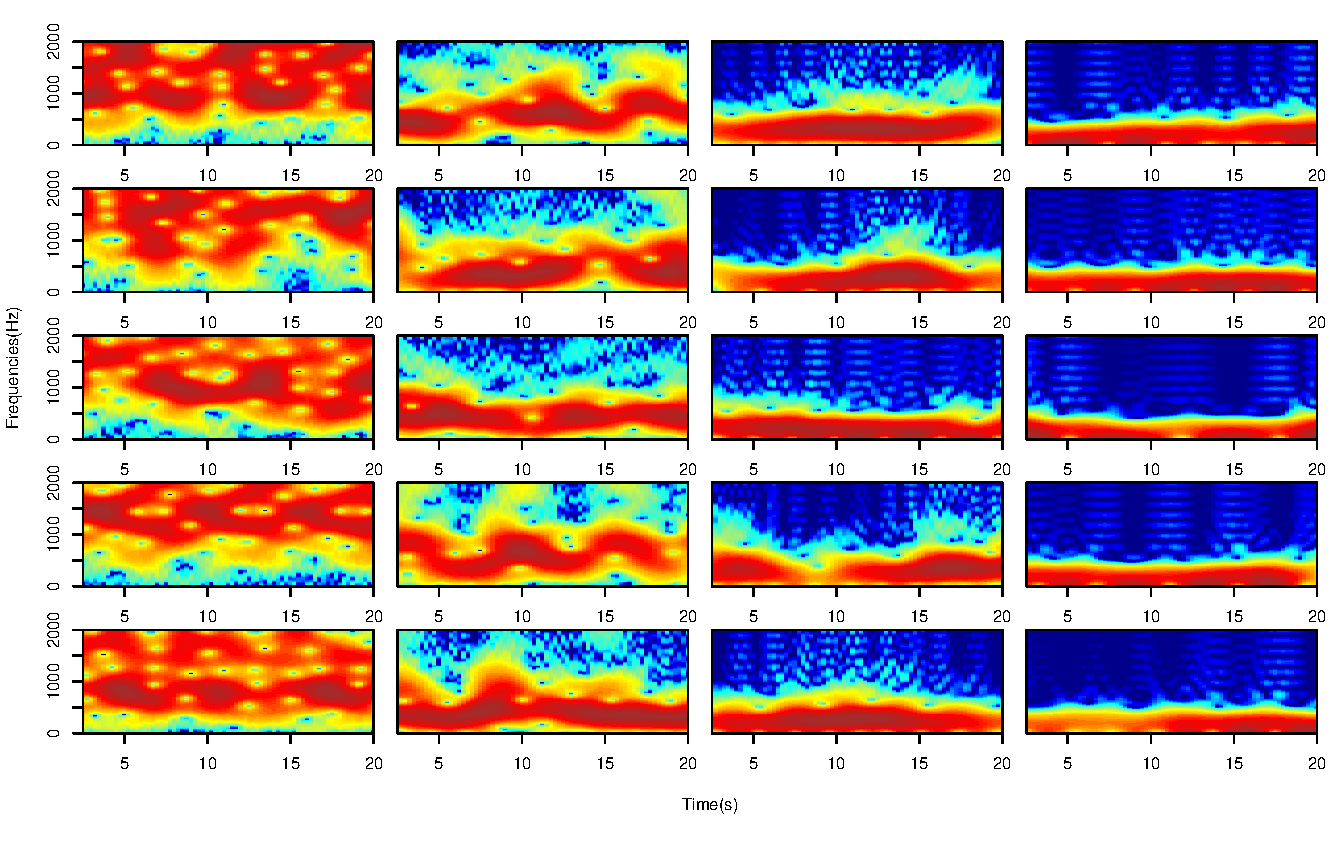
\includegraphics[width=\linewidth]{spectro_N100_l020_IMF_6_10.pdf}
%  \caption{1b}
  \label{fig:sfig2}
\end{subfigure}
\label{fig1}
\caption{$N = 100$, $l = 0.2$, $p = 0.25, 0.5, 1.00$. Spectrograms of the IMFs extracted by $\hat{x}^{(m)}$.}
\end{figure}

\restoregeometry


\newgeometry{left=2.3cm,bottom=0.1cm} 

\begin{figure}
\begin{subfigure}{1.1\textwidth}
  \centering
  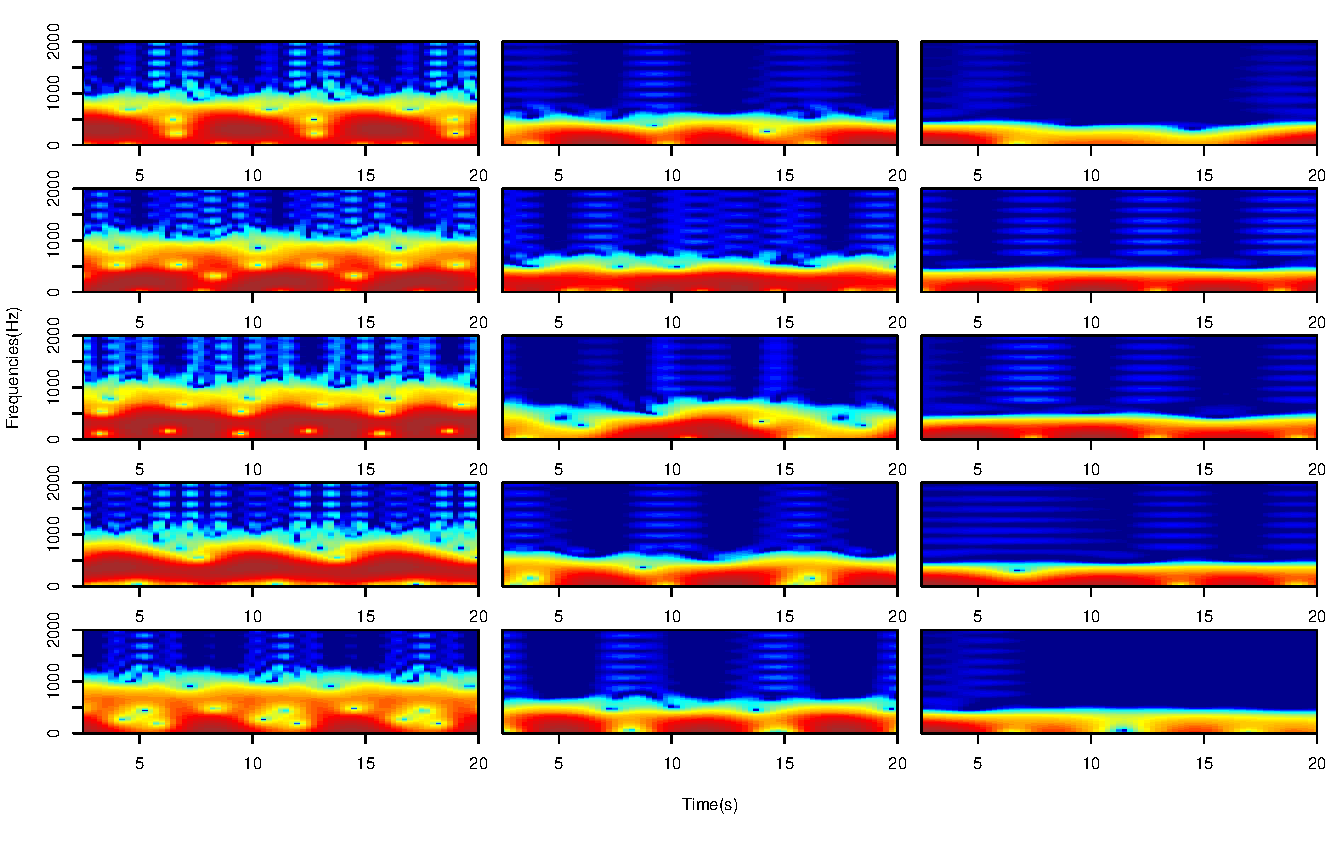
\includegraphics[width=\linewidth]{spectro_N100_l1_y_m_1_5.pdf}
%  \caption{1a}
  \label{fig:sfig1}
\end{subfigure}\\
\begin{subfigure}{1.1\textwidth}
  \centering
  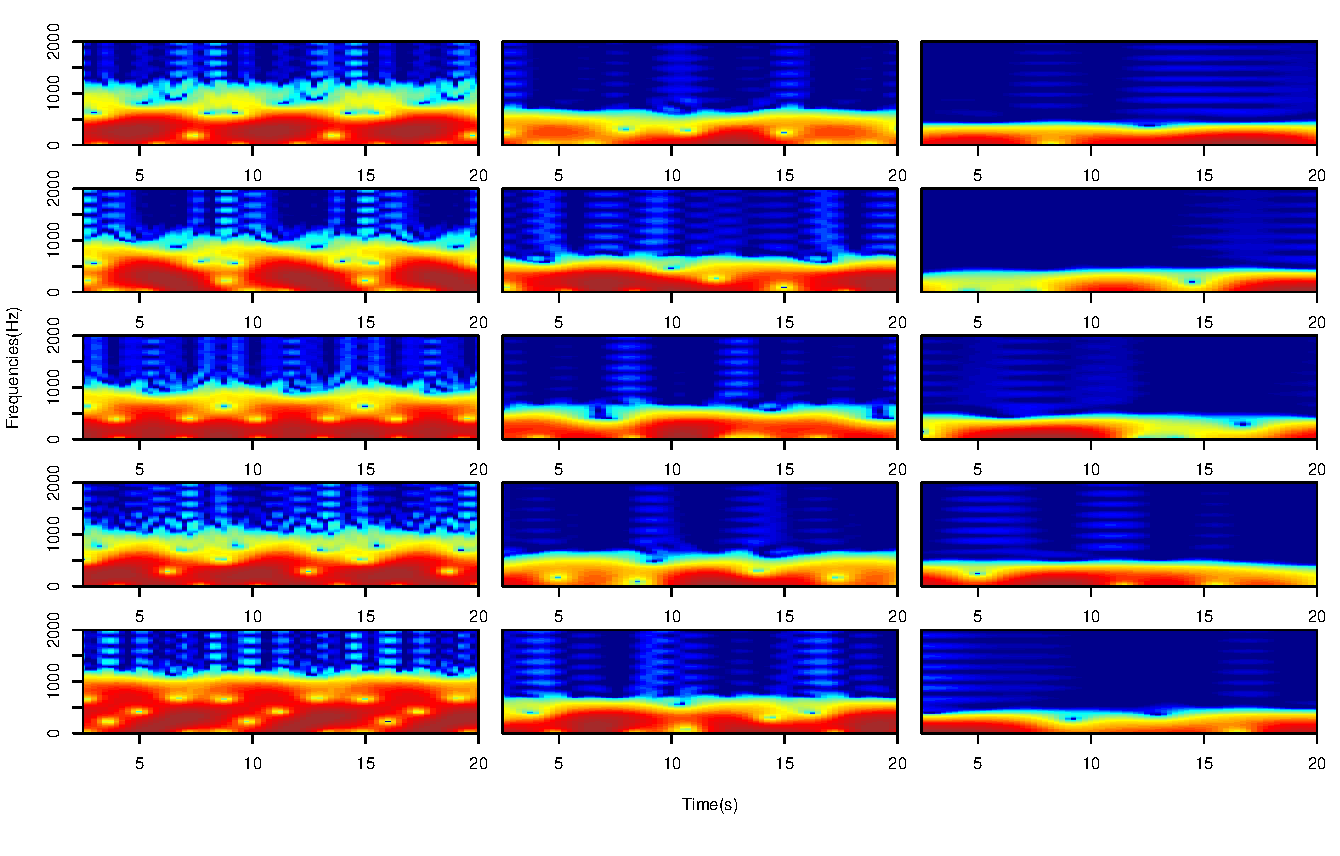
\includegraphics[width=\linewidth]{spectro_N100_l1_y_m_6_10.pdf}
%  \caption{1b}
  \label{fig:sfig2}
\end{subfigure}
\label{fig1}
\caption{$N = 100$, $l = 1$, $p = 0.25, 0.5, 1.00$. Spectrograms of the $y^{(m)}$ components.}
\end{figure}

\restoregeometry


\newgeometry{left=2.3cm,bottom=0.1cm} 

\begin{figure}
\begin{subfigure}{1.1\textwidth}
  \centering
  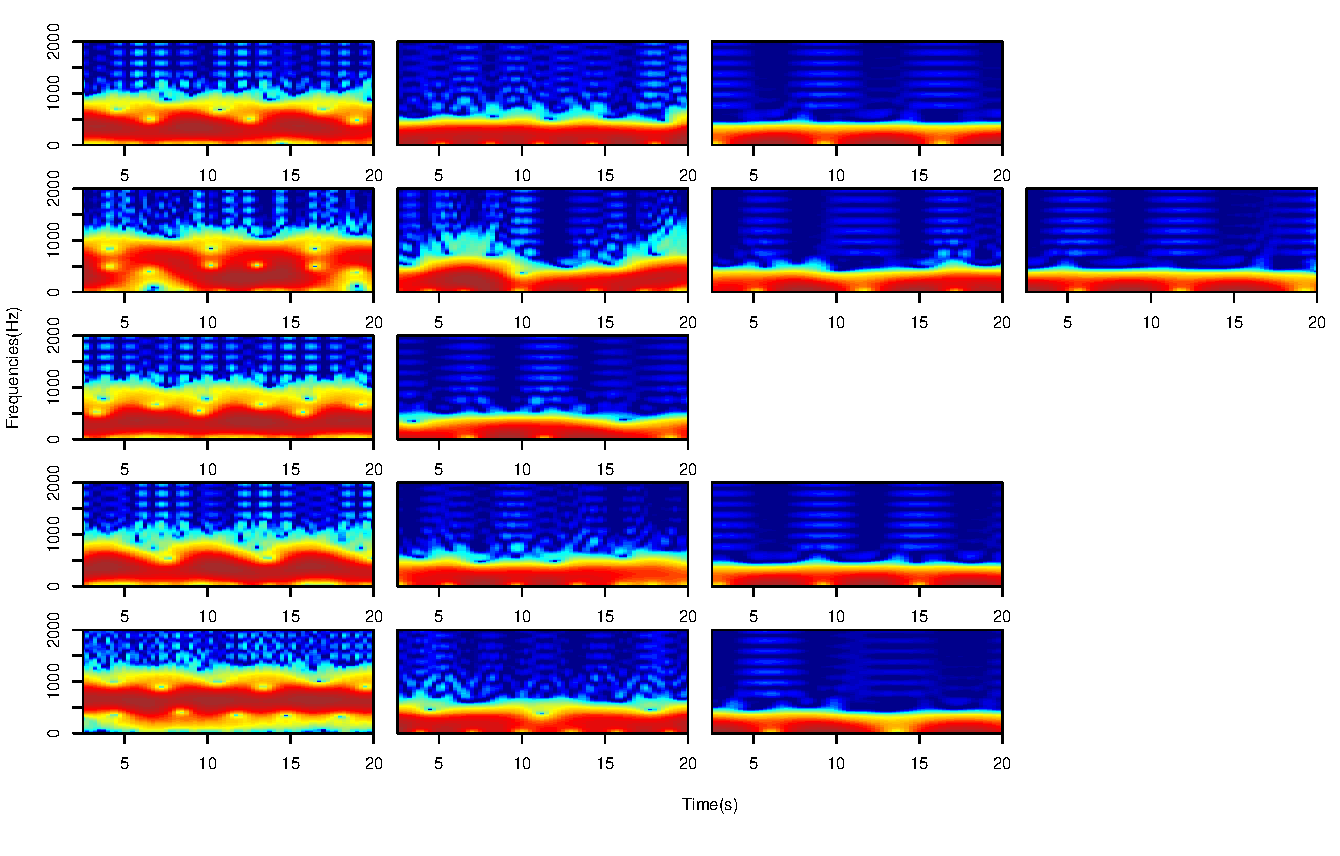
\includegraphics[width=\linewidth]{spectro_N100_l1_IMF_m_1_5.pdf}
%  \caption{1a}
  \label{fig:sfig1}
\end{subfigure}\\
\begin{subfigure}{1.1\textwidth}
  \centering
  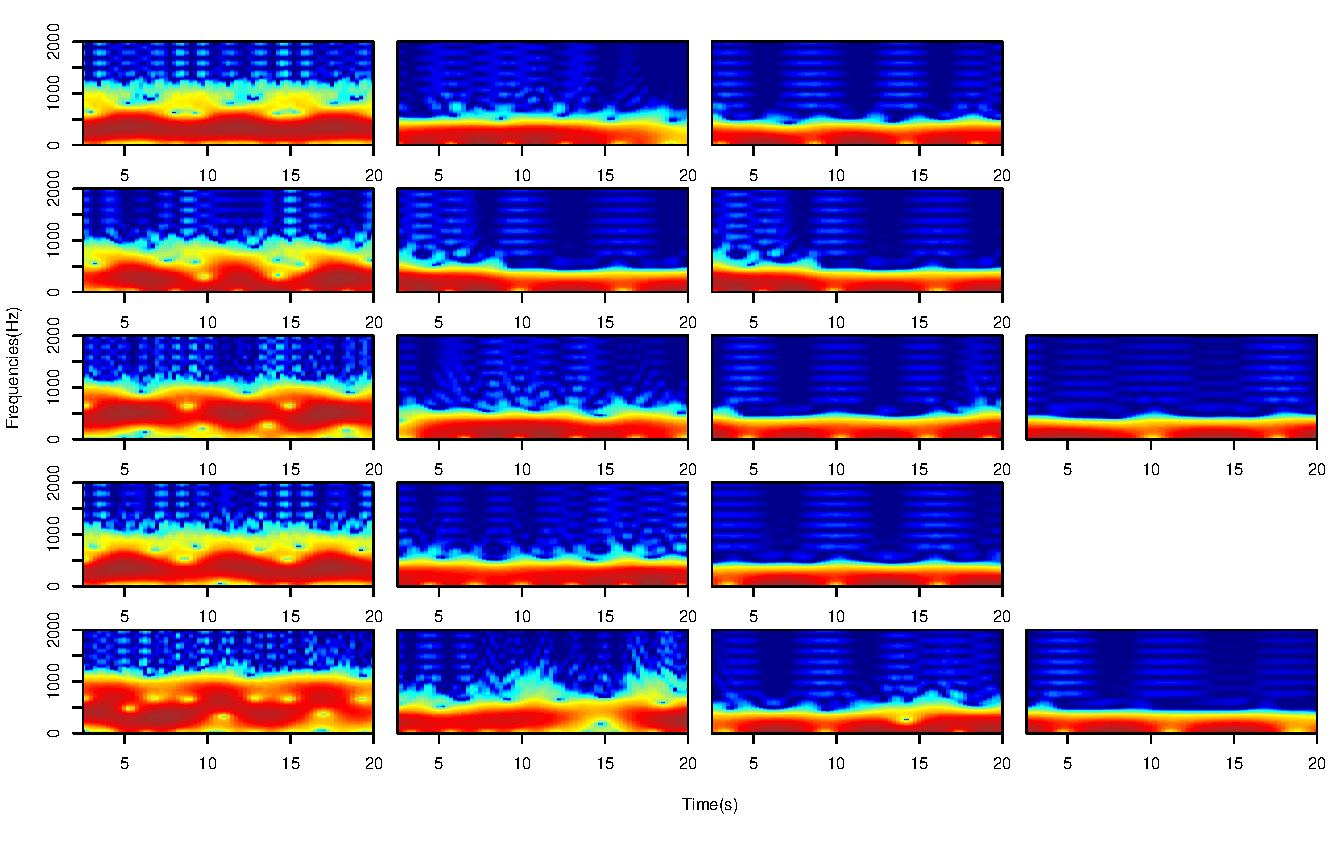
\includegraphics[width=\linewidth]{spectro_N100_l1_IMF_m_6_10.pdf}
%  \caption{1b}
  \label{fig:sfig2}
\end{subfigure}
\label{fig1}
\caption{$N = 100$, $l = 1$, $p = 0.25, 0.5, 1.00$. Spectrograms of the IMFs extracted by $\hat{x}^{(m)}$.}
\end{figure}

\restoregeometry




\newgeometry{left=2.3cm,bottom=0.1cm} 

\begin{figure}
\begin{subfigure}{1.1\textwidth}
  \centering
  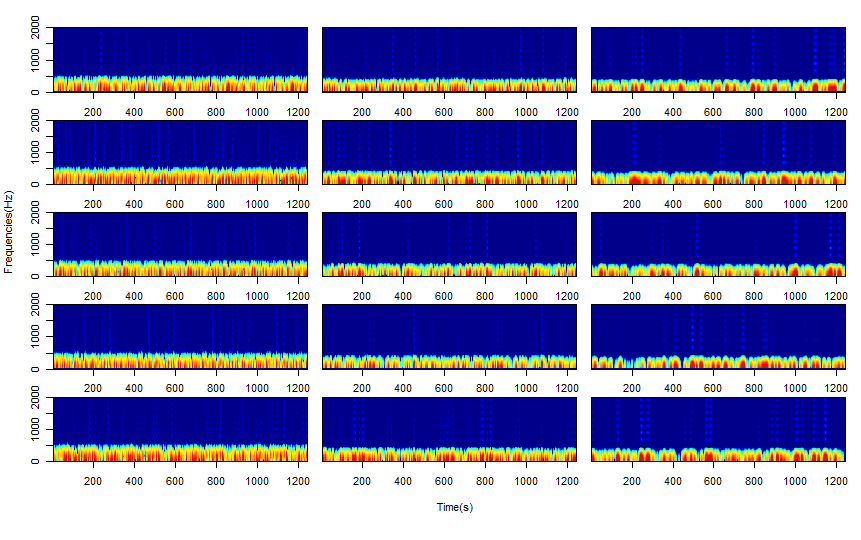
\includegraphics[width=\linewidth]{spectro_N5000_l005_y_m_1_5.png}
%  \caption{1a}
  \label{fig:sfig1}
\end{subfigure}\\
\begin{subfigure}{1.1\textwidth}
  \centering
  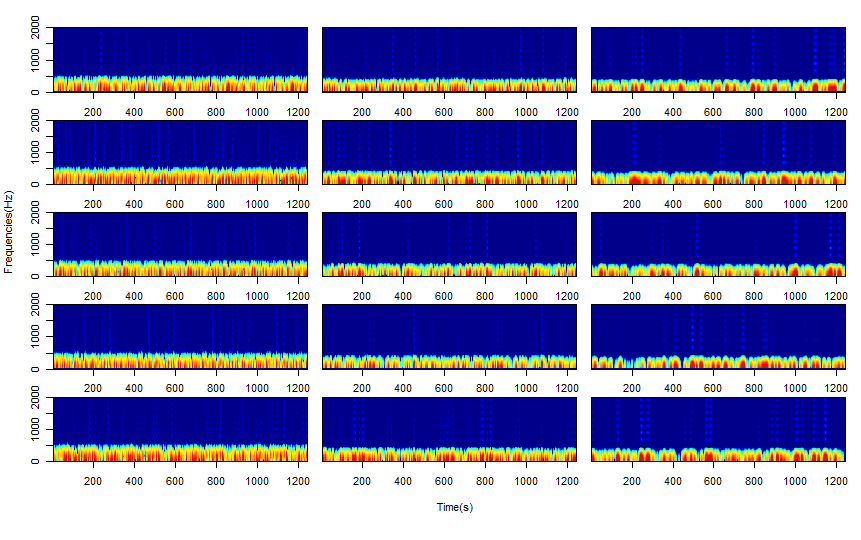
\includegraphics[width=\linewidth]{spectro_N5000_l005_IMF_m_1_5.png}
%  \caption{1b}
  \label{fig:sfig2}
\end{subfigure}
\label{fig1}
\caption{$N = 5000$, $l = 0.05$, $p = 0.25, 0.5, 1.00$. Spectrograms of the $y^{(m)}$ components and IMFs extracted by $\hat{x}^{(m)}$ for $m = 1,2,3,4,5$.}
\end{figure}

\restoregeometry


\newgeometry{left=2.3cm,bottom=0.1cm} 

\begin{figure}
\begin{subfigure}{1.1\textwidth}
  \centering
  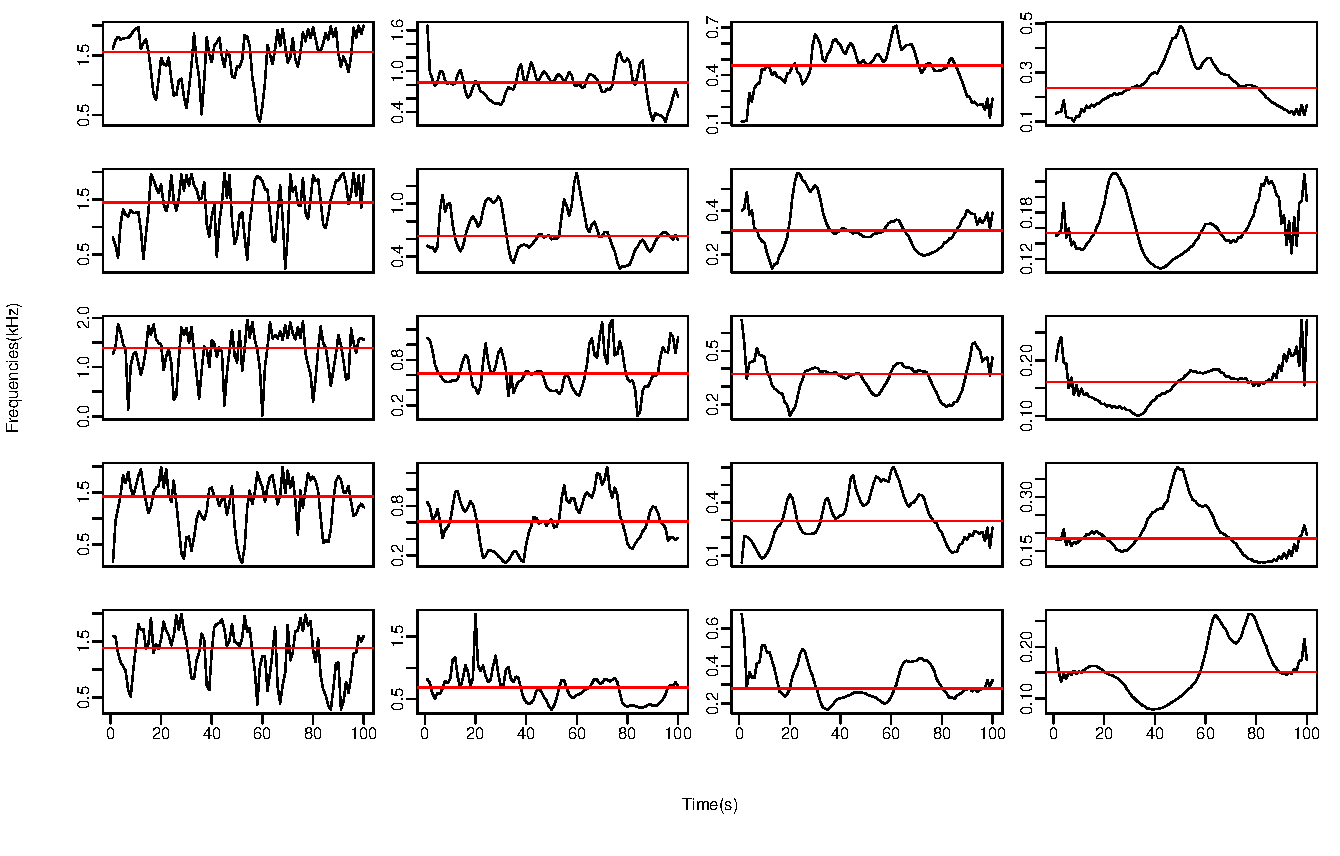
\includegraphics[width=\linewidth]{IF_N100_l005_m_1_5.pdf}
%  \caption{1a}
  \label{fig:sfig1}
\end{subfigure}\\
\begin{subfigure}{1.1\textwidth}
  \centering
  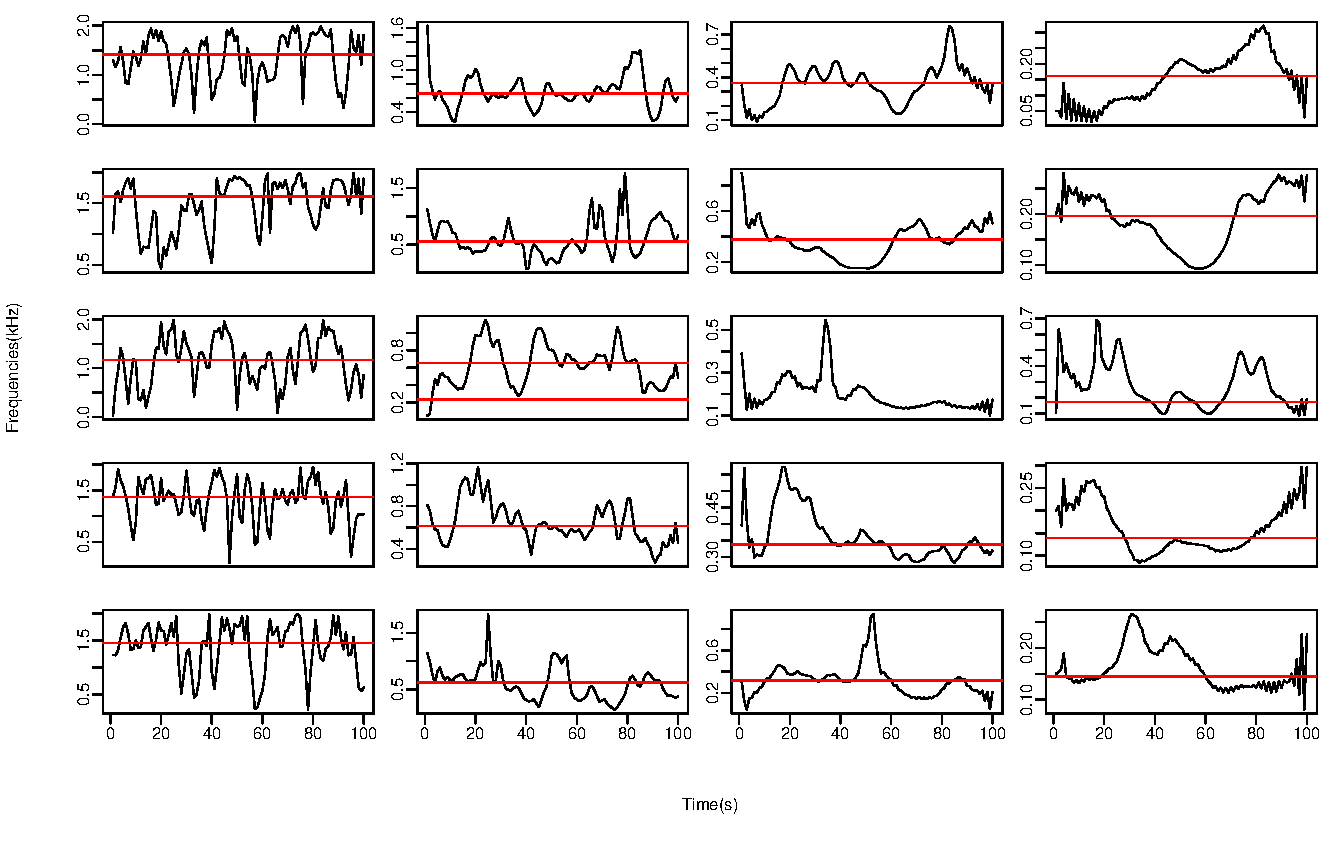
\includegraphics[width=\linewidth]{IF_N100_l005_m_6_10.pdf}
%  \caption{1b}
  \label{fig:sfig2}
\end{subfigure}
\label{fig1}
\caption{$N = 100$, $l = 0.05$, $p = 0.25, 0.5, 1.00$. Instantaneous Frequencies of the IMFs extracted by $\hat{x}^{(m)}$.}
\end{figure}

\restoregeometry


\newgeometry{left=2.3cm,bottom=0.1cm} 

\begin{figure}
\begin{subfigure}{1.1\textwidth}
  \centering
  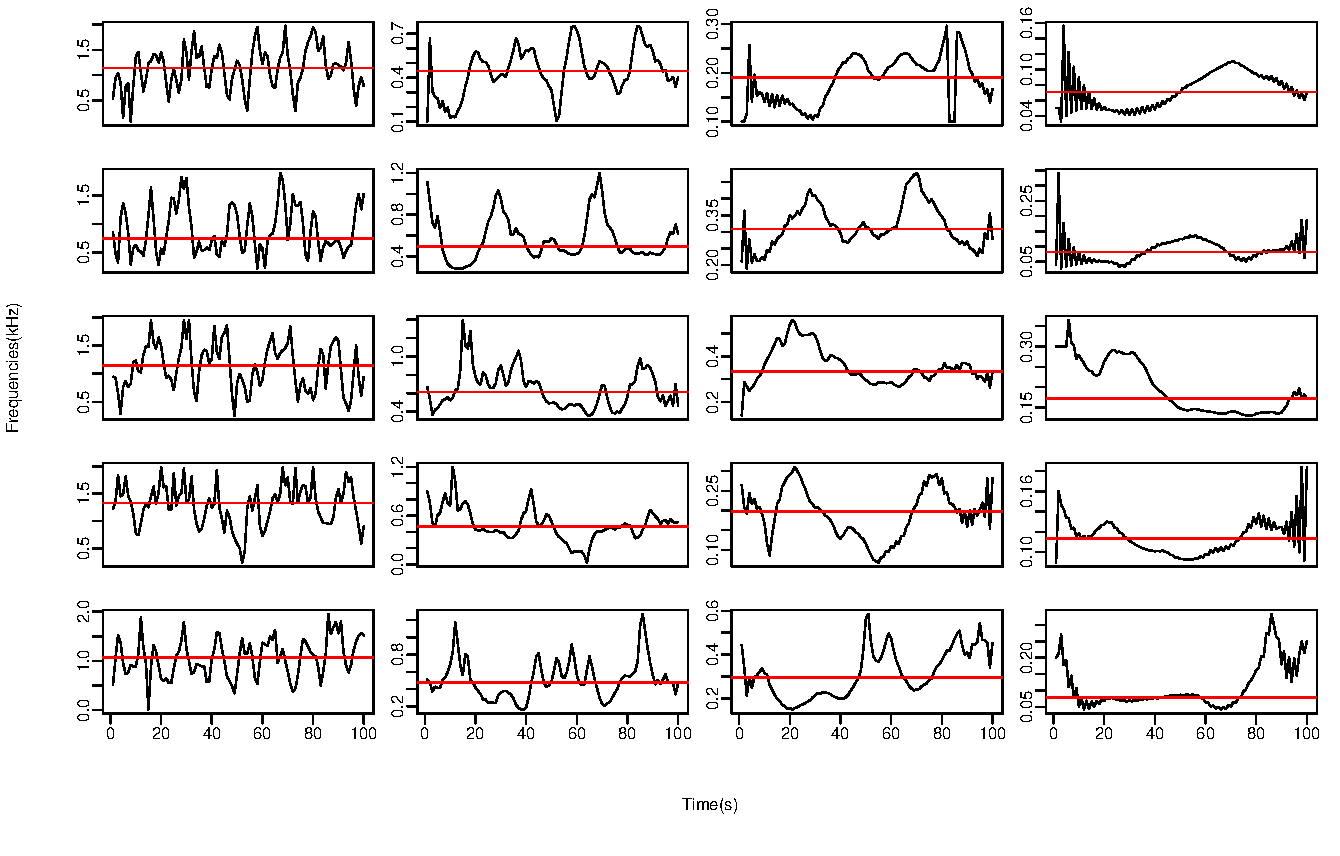
\includegraphics[width=\linewidth]{IF_N100_l02_m_1_5.pdf}
%  \caption{1a}
  \label{fig:sfig1}
\end{subfigure}\\
\begin{subfigure}{1.1\textwidth}
  \centering
  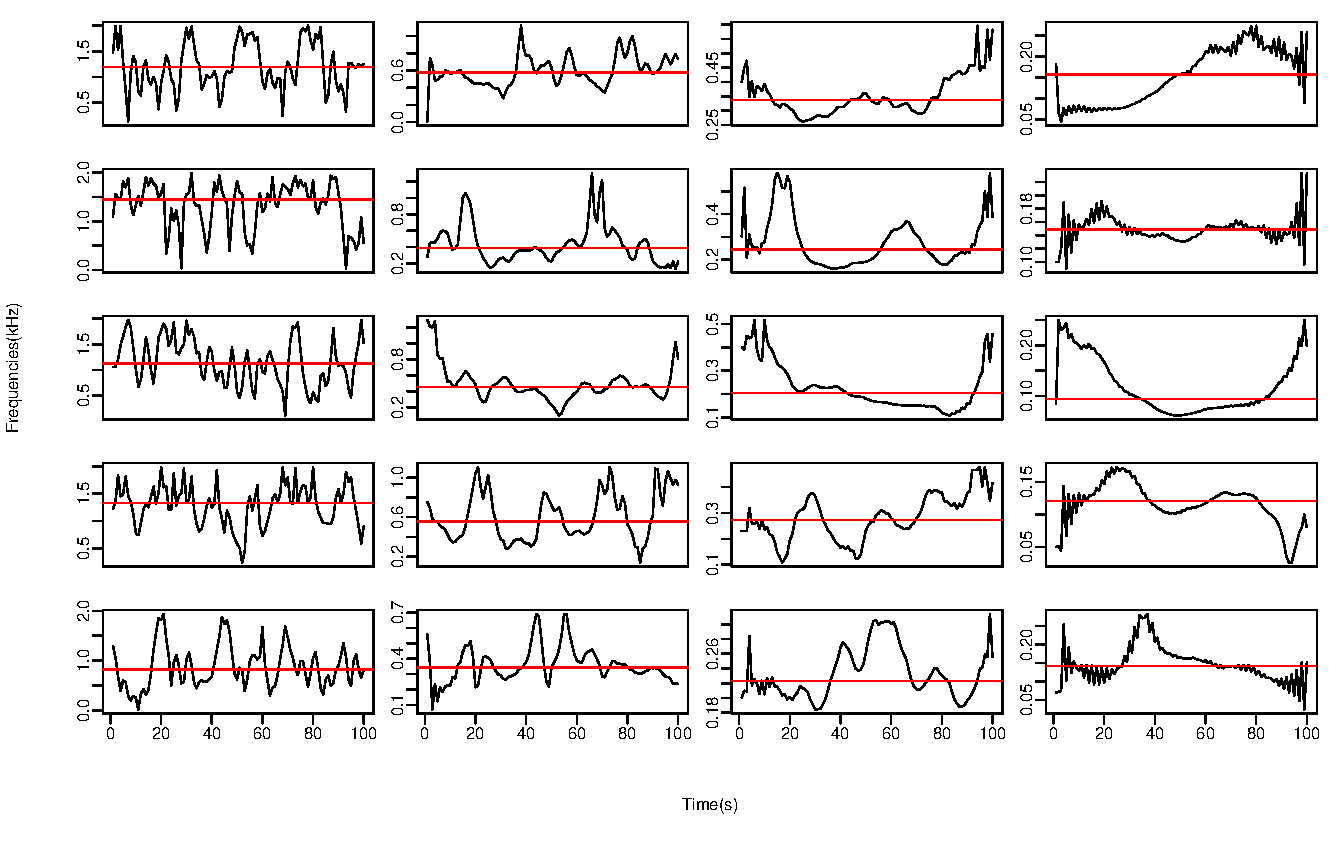
\includegraphics[width=\linewidth]{IF_N100_l02_m_6_10.pdf}
%  \caption{1b}
  \label{fig:sfig2}
\end{subfigure}
\label{fig1}
\caption{$N = 100$, $l = 0.2$, $p = 0.25, 0.5, 1.00$. Instantaneous Frequencies of the IMFs extracted by $\hat{x}^{(m)}$.}
\end{figure}

\restoregeometry


\newgeometry{left=2.3cm,bottom=0.1cm} 

\begin{figure}
\begin{subfigure}{1.1\textwidth}
  \centering
  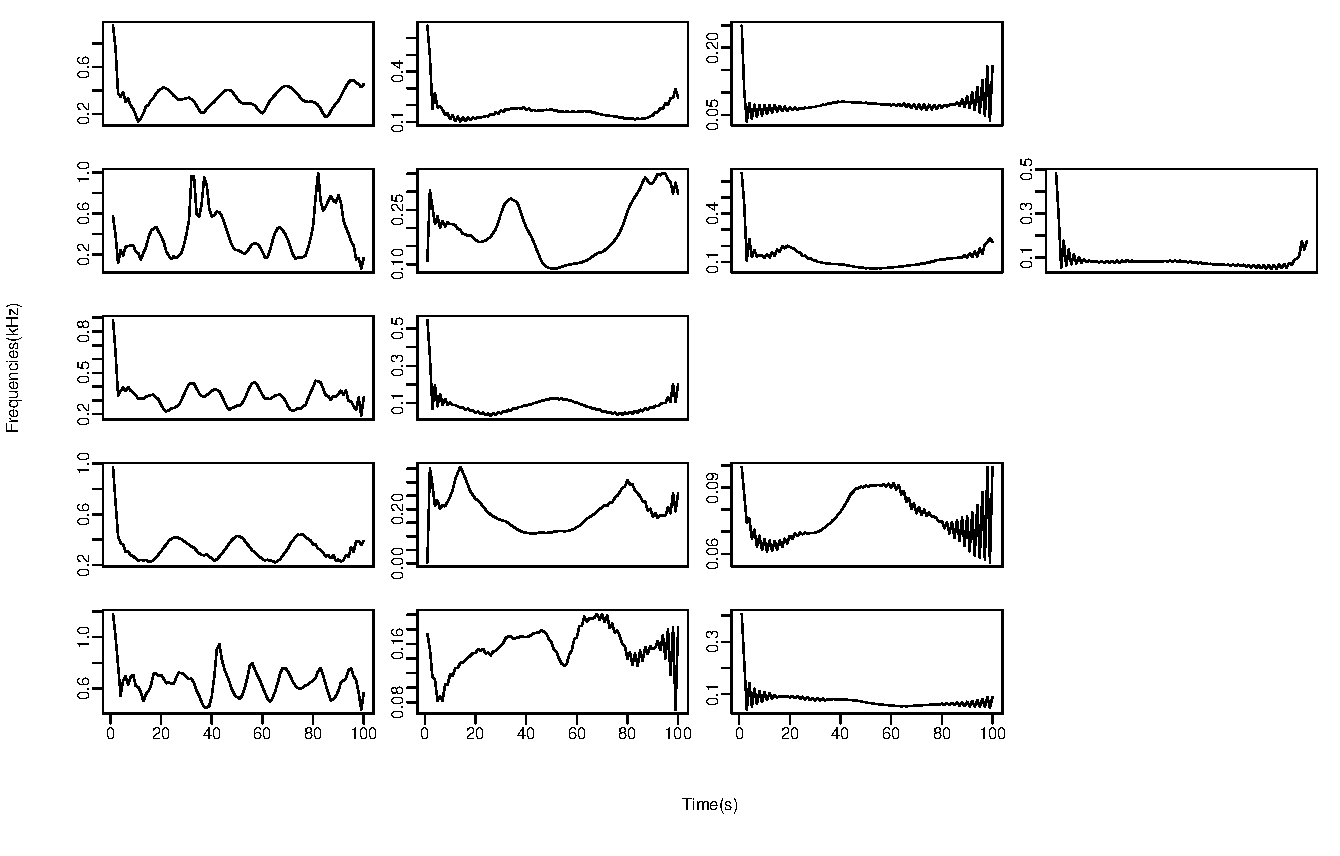
\includegraphics[width=\linewidth]{IF_N100_l1_m_1_5.pdf}
%  \caption{1a}
  \label{fig:sfig1}
\end{subfigure}\\
\begin{subfigure}{1.1\textwidth}
  \centering
  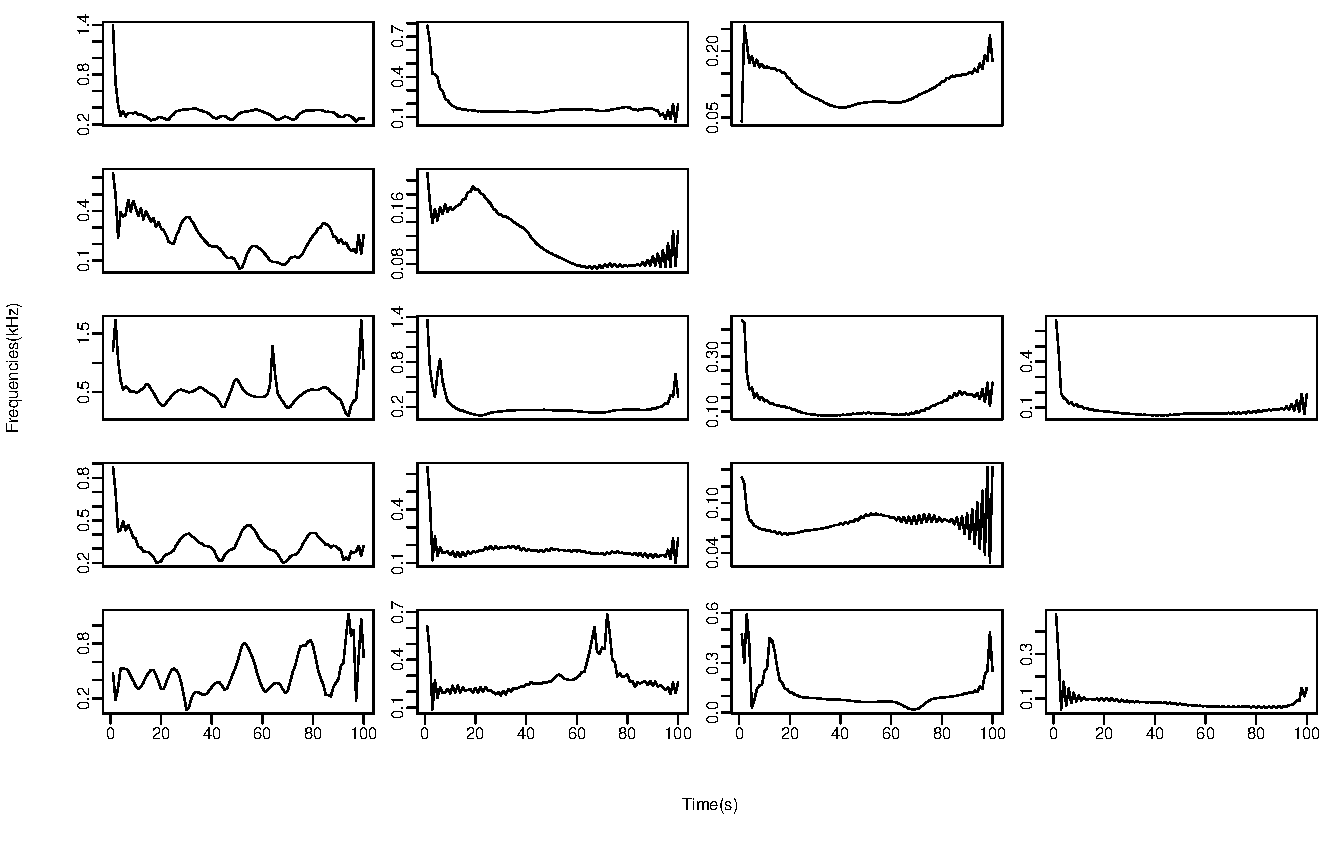
\includegraphics[width=\linewidth]{IF_N100_l1_m_6_10.pdf}
%  \caption{1b}
  \label{fig:sfig2}
\end{subfigure}
\label{fig1}
\caption{$N = 100$, $l = 1$, $p = 0.25, 0.5, 1.00$. Instantaneous Frequencies of the IMFs extracted by $\hat{x}^{(m)}$.}
\end{figure}

\restoregeometry



\newgeometry{left=2.3cm,bottom=0.1cm} 

\begin{figure}
\begin{subfigure}{1.1\textwidth}
  \centering
  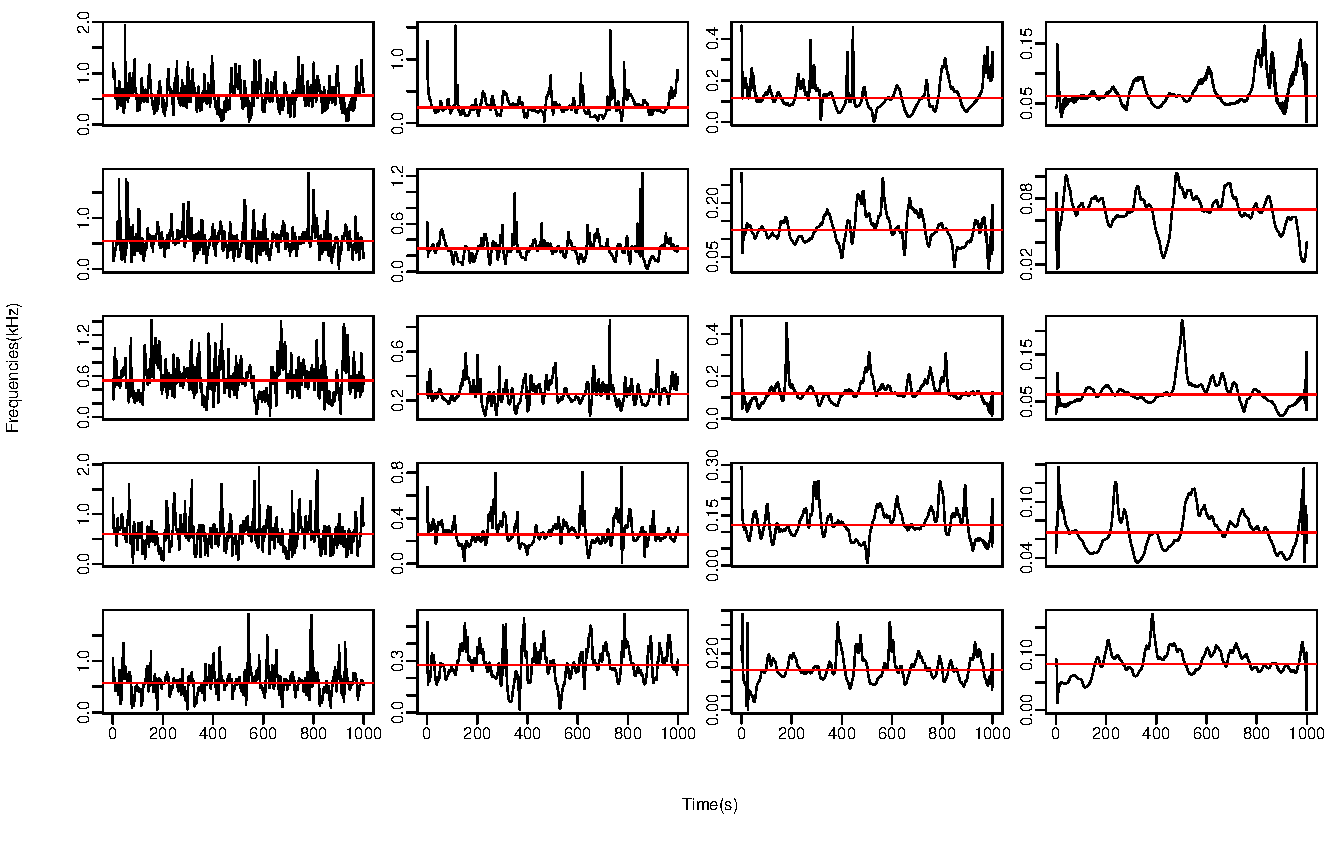
\includegraphics[width=\linewidth]{IF_N1000_l005_m1_5.pdf}
%  \caption{1a}
  \label{fig:sfig1}
\end{subfigure}\\
\begin{subfigure}{1.1\textwidth}
  \centering
  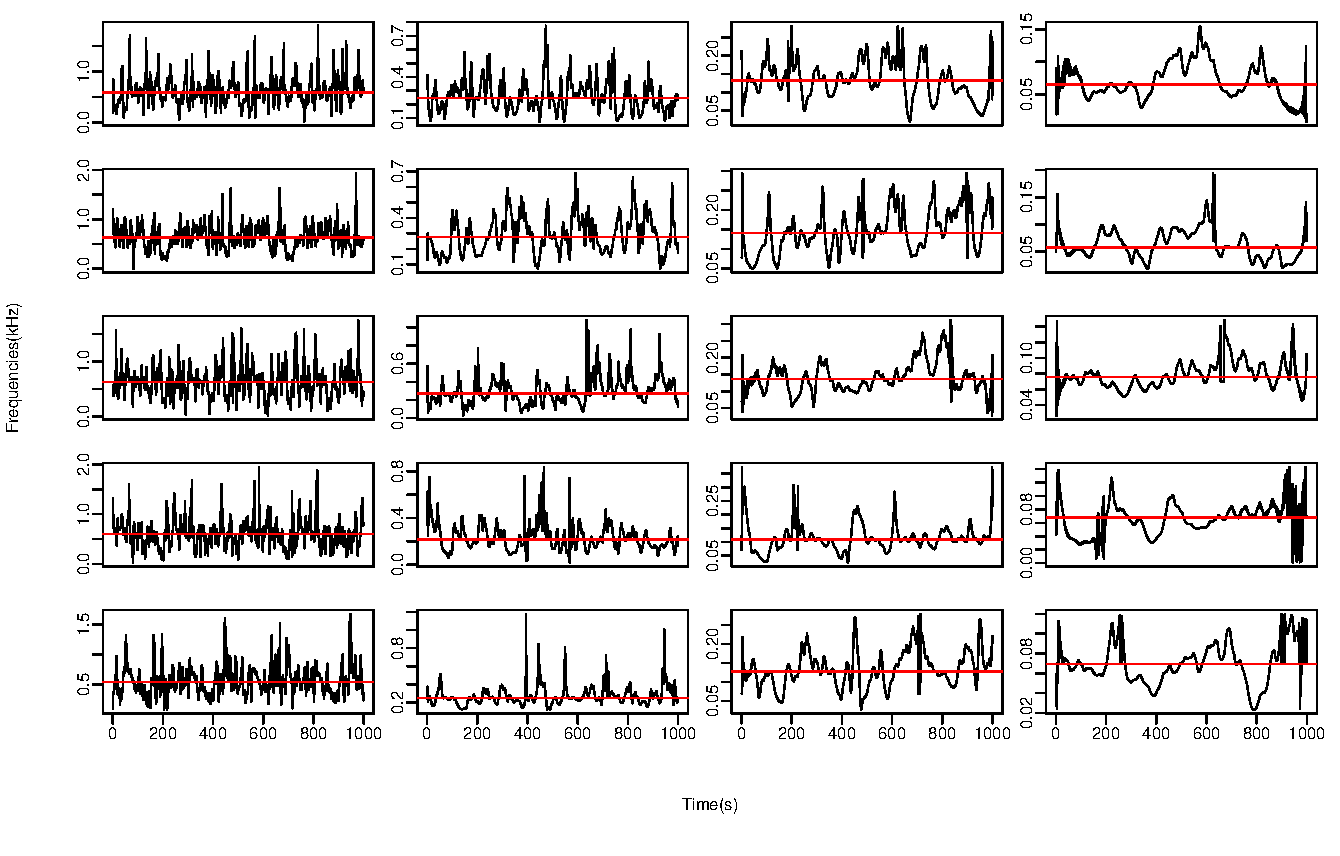
\includegraphics[width=\linewidth]{IF_N1000_l005_m6_10.pdf}
%  \caption{1b}
  \label{fig:sfig2}
\end{subfigure}
\label{fig1}
\caption{$N = 1000$, $l = 0.05$, $p = 0.25, 0.5, 1.00$. Instantaneous Frequencies of the IMFs extracted by $\hat{x}^{(m)}$.}
\end{figure}

\restoregeometry



\newgeometry{left=2.3cm,bottom=0.1cm} 

\begin{figure}
\begin{subfigure}{1.1\textwidth}
  \centering
  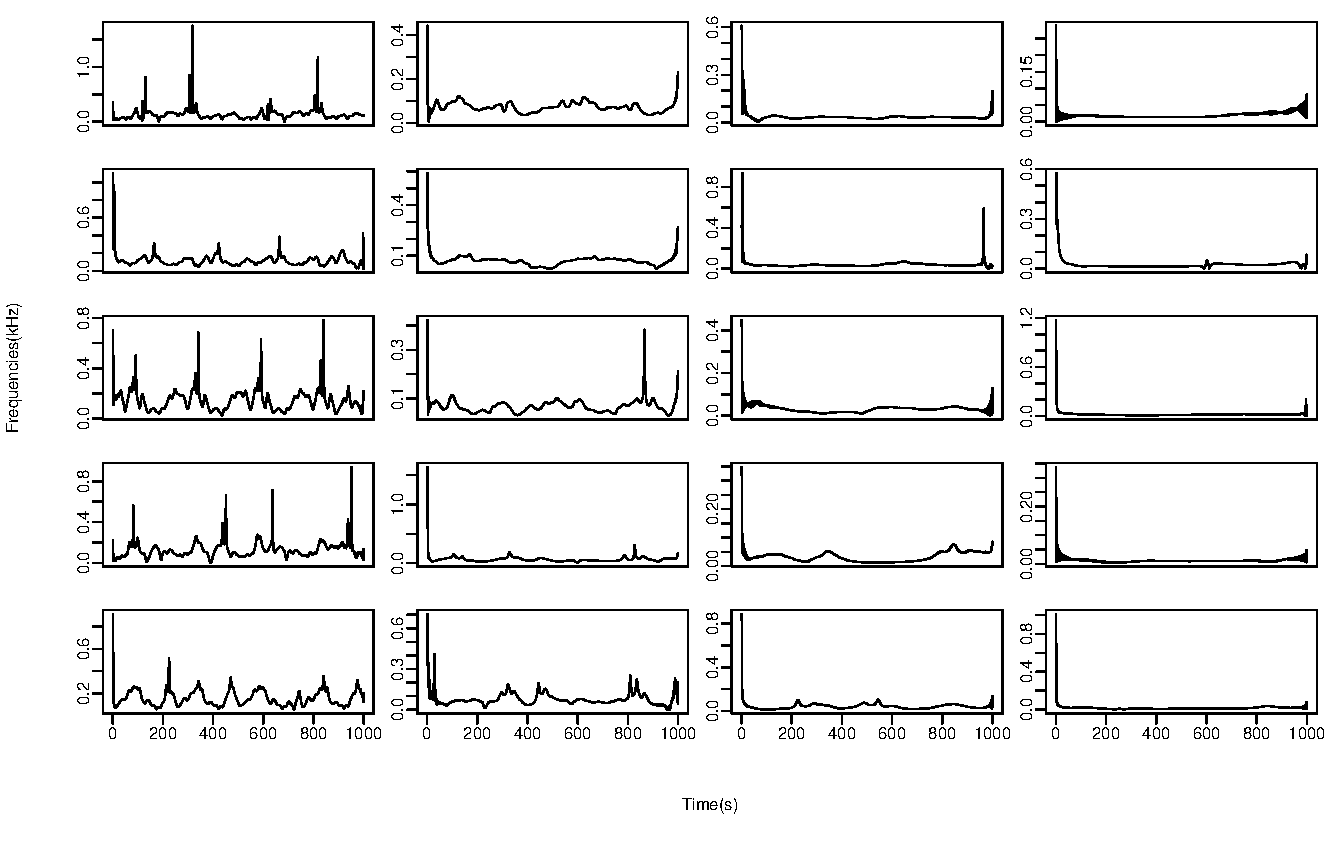
\includegraphics[width=\linewidth]{IF_N1000_l020_m_1_5.pdf}
%  \caption{1a}
  \label{fig:sfig1}
\end{subfigure}\\
\begin{subfigure}{1.1\textwidth}
  \centering
  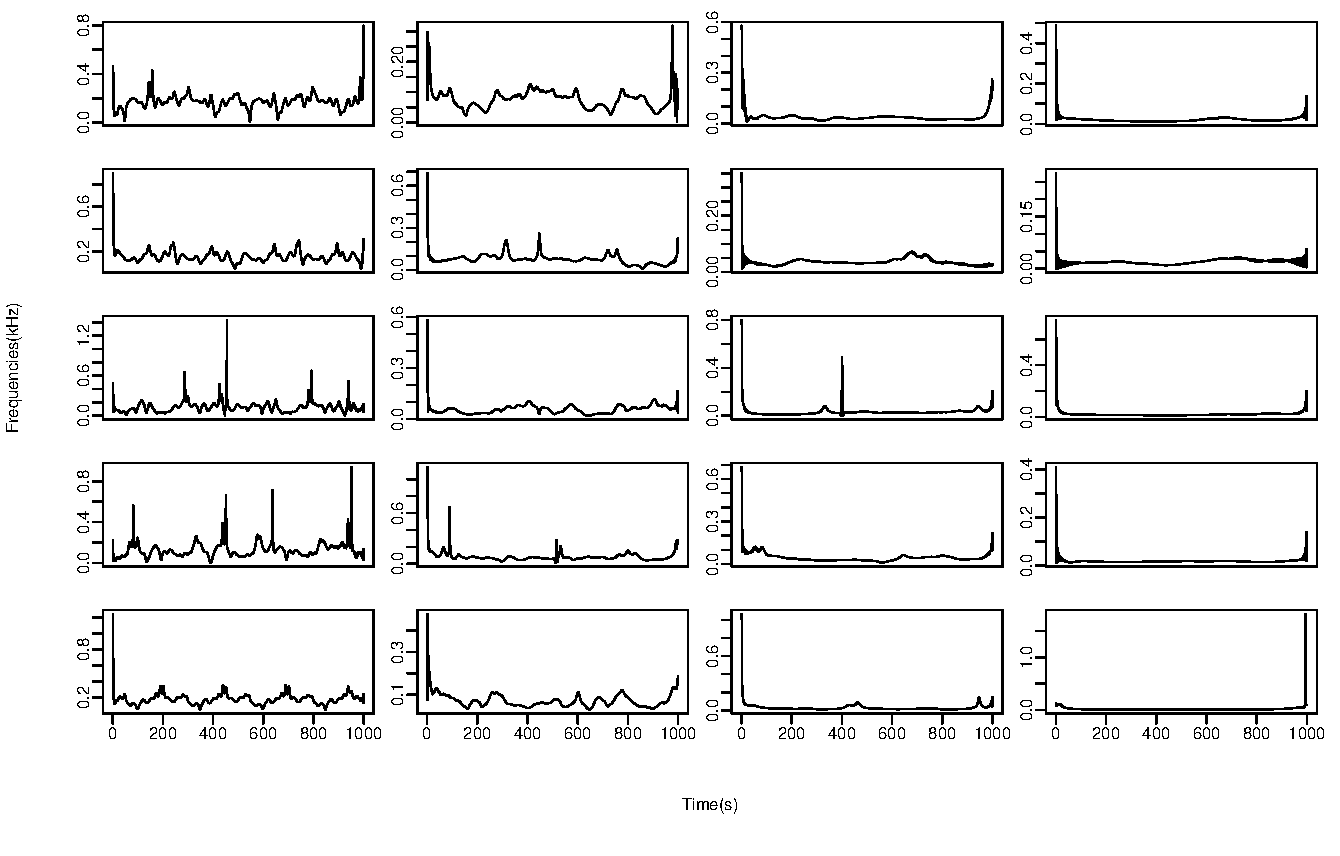
\includegraphics[width=\linewidth]{IF_N1000_l020_m_6_10.pdf}
%  \caption{1b}
  \label{fig:sfig2}
\end{subfigure}
\label{fig1}
\caption{$N = 1000$, $l = 0.2$, $p = 0.25, 0.5, 1.00$. Instantaneous Frequencies of the IMFs extracted by $\hat{x}^{(m)}$.}
\end{figure}

\restoregeometry



\newgeometry{left=2.3cm,bottom=0.1cm} 

\begin{figure}
\begin{subfigure}{1.1\textwidth}
  \centering
  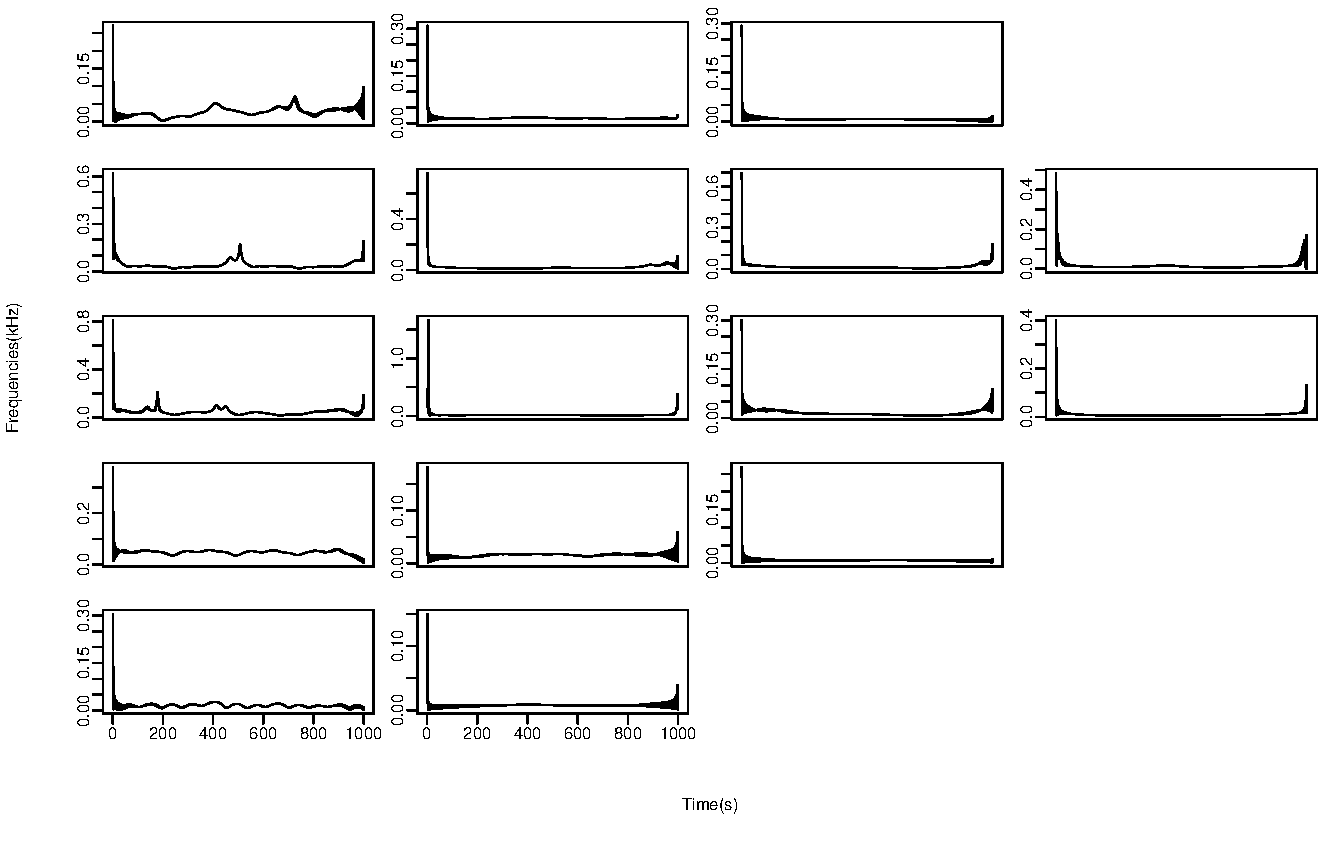
\includegraphics[width=\linewidth]{IF_N1000_l1_m1_5.pdf}
%  \caption{1a}
  \label{fig:sfig1}
\end{subfigure}\\
\begin{subfigure}{1.1\textwidth}
  \centering
  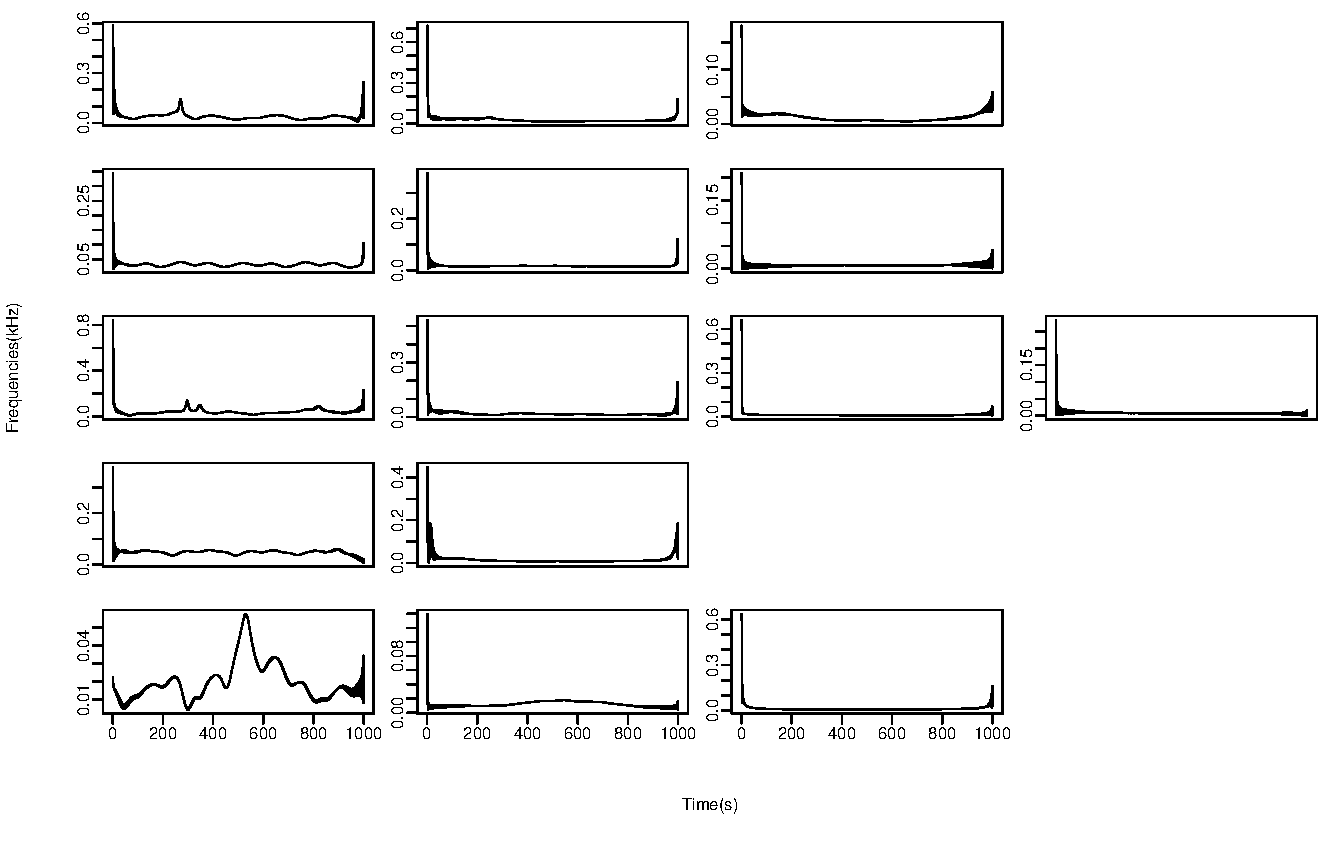
\includegraphics[width=\linewidth]{IF_N1000_l1_m6_10.pdf}
%  \caption{1b}
  \label{fig:sfig2}
\end{subfigure}
\label{fig1}
\caption{$N = 1000$, $l =1$, $p = 0.25, 0.5, 1.00$. Instantaneous Frequencies of the IMFs extracted by $\hat{x}^{(m)}$.}
\end{figure}

\restoregeometry


\newgeometry{left=2.3cm,bottom=0.1cm} 

\begin{figure}
\begin{subfigure}{1.1\textwidth}
  \centering
  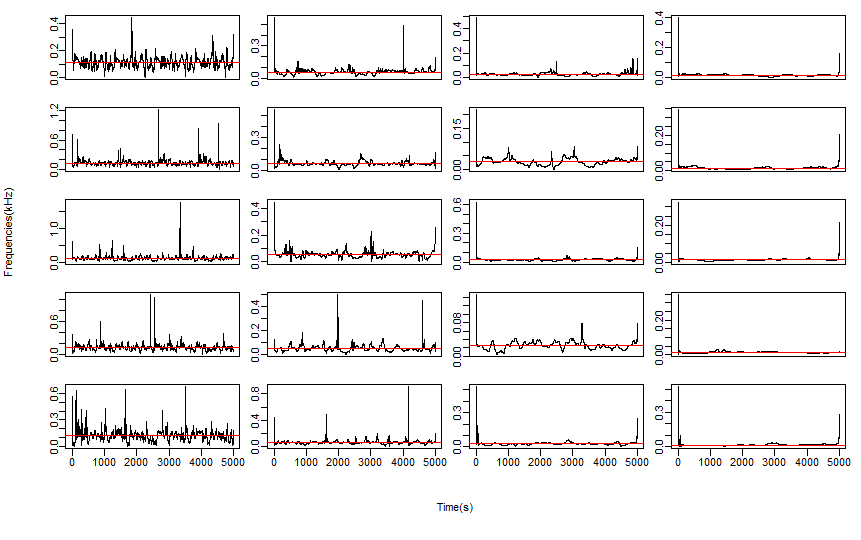
\includegraphics[width=\linewidth]{IF_N5000_l005_m_1_5.png}
%  \caption{1a}
  \label{fig:sfig1}
\end{subfigure}\\
\label{fig1}
\caption{$N = 5000$, $l =0.05$, $p = 0.25, 0.5, 1.00$. Instantaneous Frequencies of the IMFs extracted by $\hat{x}^{(m)}$, $m = 1,2,3,4,5$.}
\end{figure}

\restoregeometry




\newgeometry{left=2.3cm,bottom=0.1cm} 

\begin{figure}
\begin{subfigure}{1.1\textwidth}
  \centering
  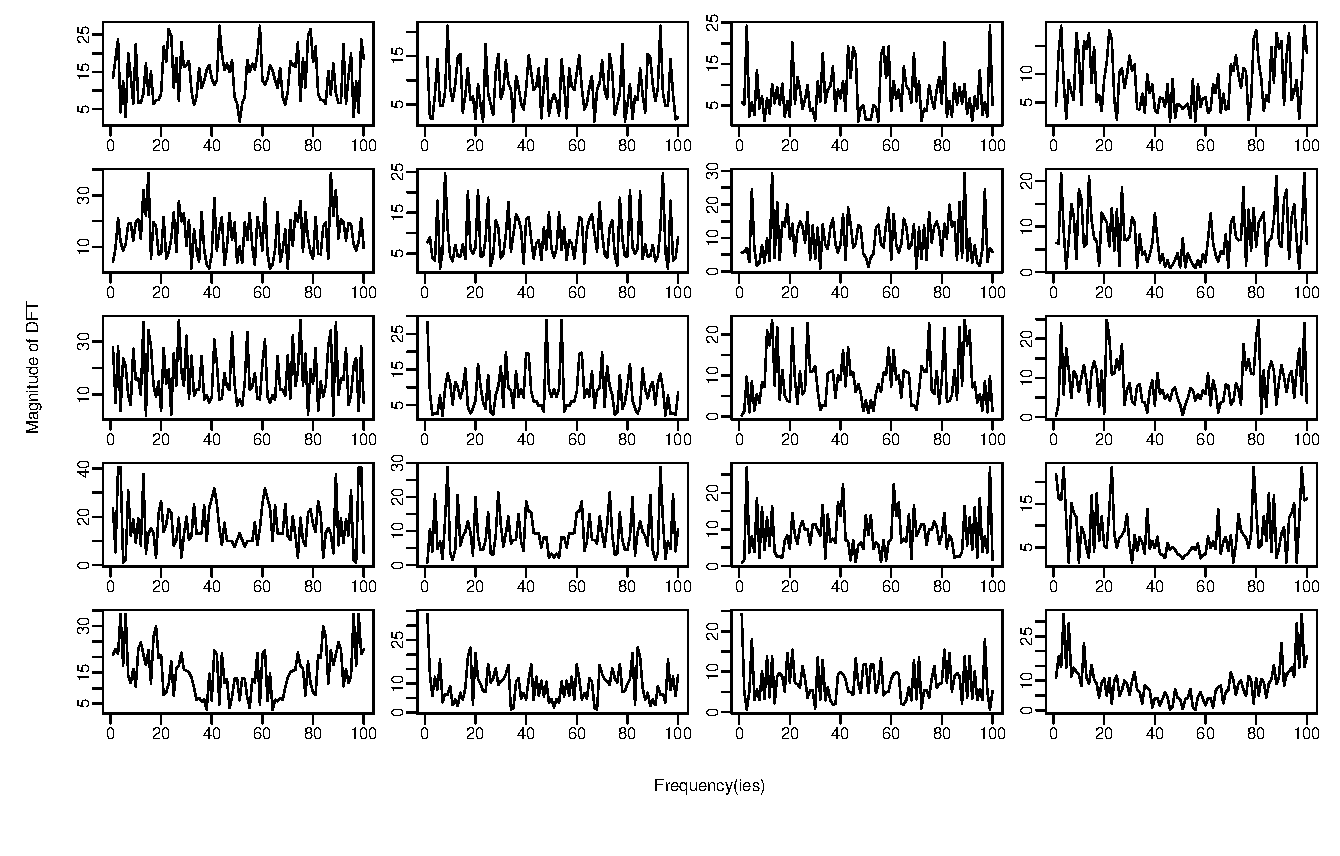
\includegraphics[width=\linewidth]{N100_MagnDFT_l005_m_1_5.pdf}
%  \caption{1a}
  \label{fig:sfig1}
\end{subfigure}\\
\begin{subfigure}{1.1\textwidth}
  \centering
  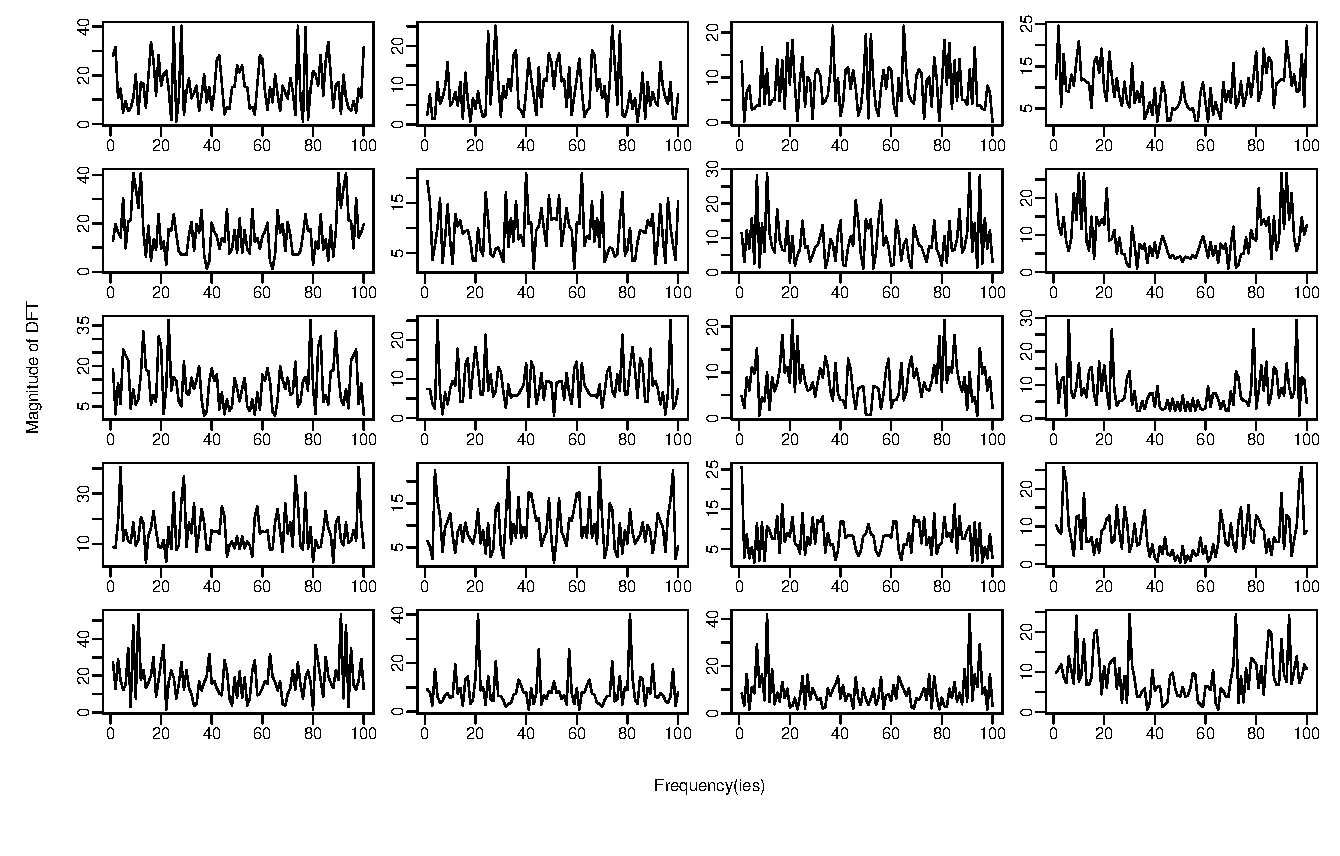
\includegraphics[width=\linewidth]{N100_MagnDFT_l005_m_6_10.pdf}
%  \caption{1b}
  \label{fig:sfig2}
\end{subfigure}
\label{fig1}
\caption{$N = 100$, $l =0.05$, $p = 0.25, 0.5, 1.00$. Magnitudes of the DFT, $m = 1,2, \dots, 10$.}
\end{figure}

\restoregeometry




\newgeometry{left=2.3cm,bottom=0.1cm} 

\begin{figure}
\begin{subfigure}{1.1\textwidth}
  \centering
  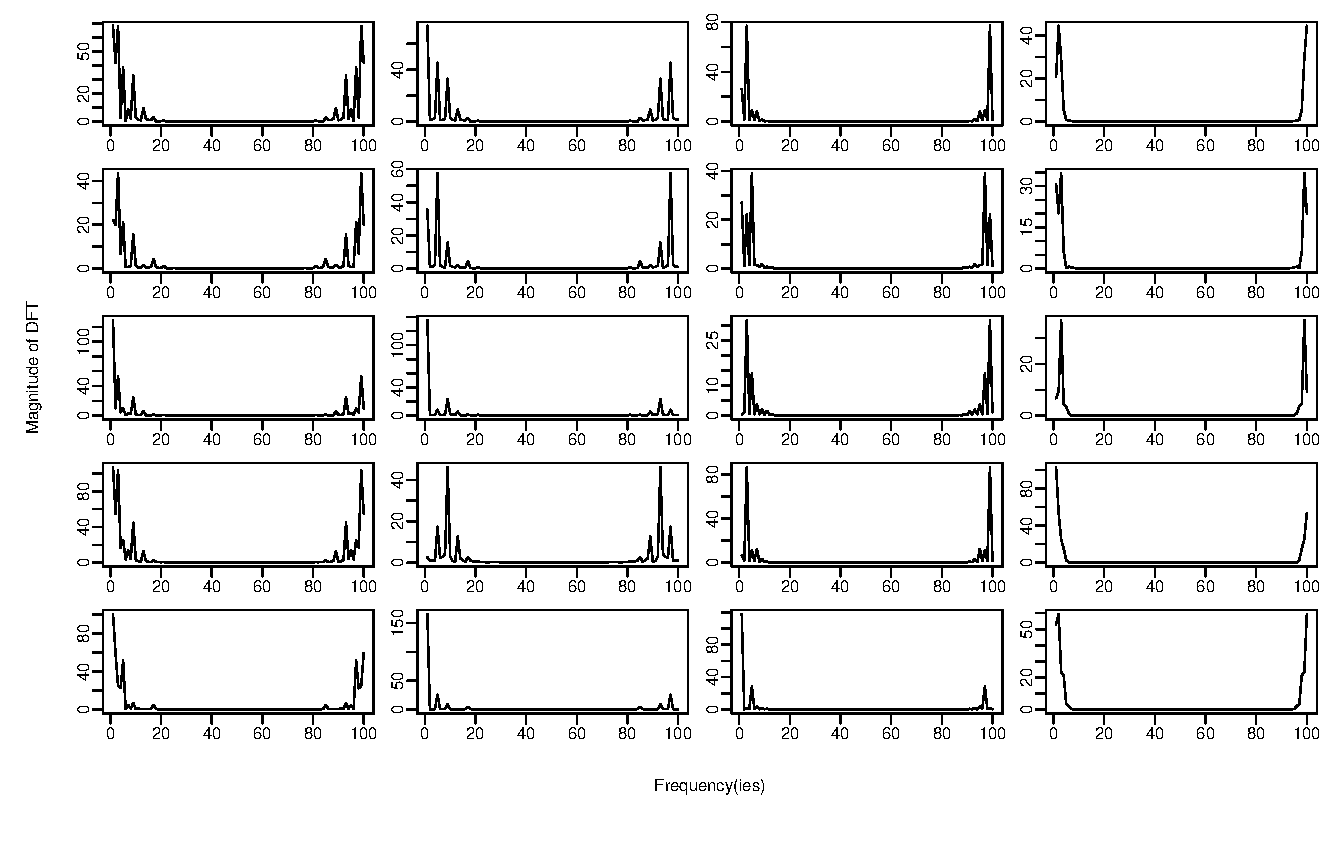
\includegraphics[width=\linewidth]{N100_MagnDFT_l1_m_1_5.pdf}
%  \caption{1a}
  \label{fig:sfig1}
\end{subfigure}\\
\begin{subfigure}{1.1\textwidth}
  \centering
  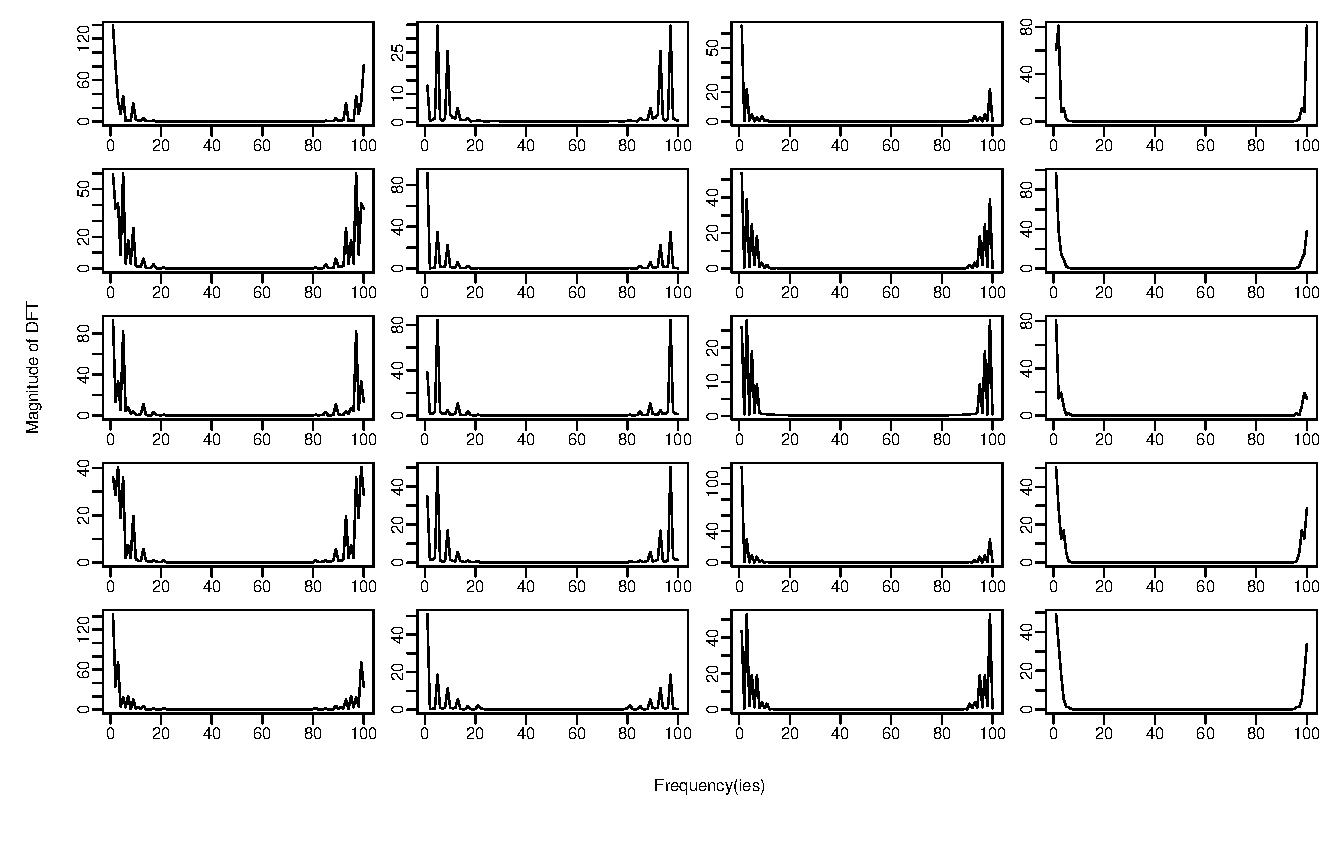
\includegraphics[width=\linewidth]{N100_MagnDFT_l1_m_6_10.pdf}
%  \caption{1b}
  \label{fig:sfig2}
\end{subfigure}
\label{fig1}
\caption{$N = 100$, $l =1$, $p = 0.25, 0.5, 1.00$. Magnitudes of the DFT, $m = 1,2, \dots, 10$.}
\end{figure}

\restoregeometry


\newgeometry{left=2.3cm,bottom=0.1cm} 

\begin{figure}
\begin{subfigure}{1.1\textwidth}
  \centering
  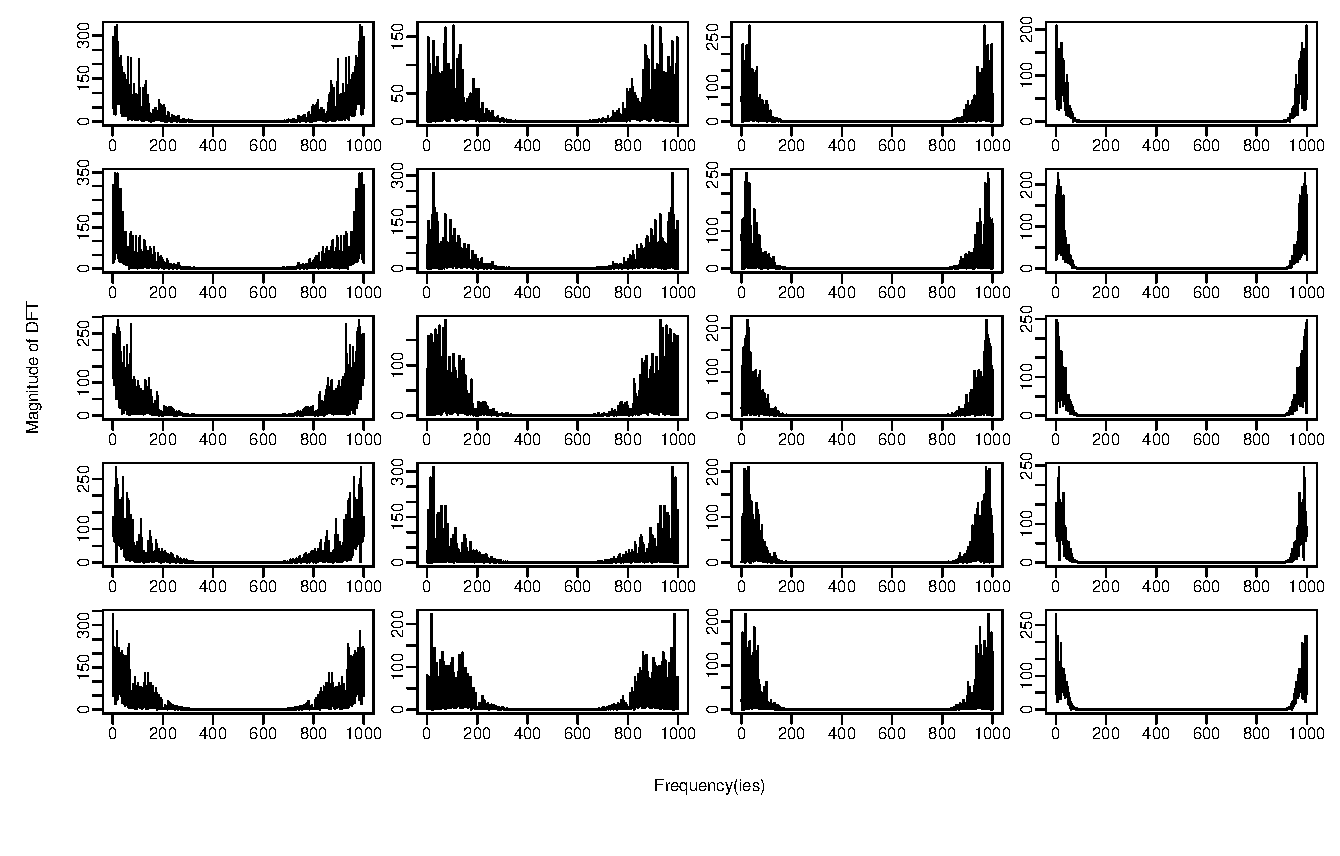
\includegraphics[width=\linewidth]{N1000_MagnDFT_l005_m_1_5.pdf}
%  \caption{1a}
  \label{fig:sfig1}
\end{subfigure}\\
\begin{subfigure}{1.1\textwidth}
  \centering
  \includegraphics[width=\linewidth]{N1000_MagnDFT_l005_m_6_10.pdf}
%  \caption{1b}
  \label{fig:sfig2}
\end{subfigure}
\label{fig1}
\caption{$N = 1000$, $l =0.05$, $p = 0.25, 0.5, 1.00$. Magnitudes of the DFT, $m = 1,2, \dots, 10$.}
\end{figure}

\restoregeometry


\newgeometry{left=2.3cm,bottom=0.1cm} 

\begin{figure}
\begin{subfigure}{1.1\textwidth}
  \centering
  \includegraphics[width=\linewidth]{N1000_MagnDFT_l1_m_1_5.pdf}
%  \caption{1a}
  \label{fig:sfig1}
\end{subfigure}\\
\begin{subfigure}{1.1\textwidth}
  \centering
  \includegraphics[width=\linewidth]{N1000_MagnDFT_l1_m_6_10.pdf}
%  \caption{1b}
  \label{fig:sfig2}
\end{subfigure}
\label{fig1}
\caption{$N = 1000$, $l = 1$, $p = 0.25, 0.5, 1.00$. Magnitudes of the DFT, $m = 1,2, \dots, 10$.}
\end{figure}

\restoregeometry


\newgeometry{left=2.3cm,bottom=0.1cm} 

\begin{figure}
\begin{subfigure}{1.1\textwidth}
  \centering
  \includegraphics[width=\linewidth]{N100_MagnDFT_p025_l005001015_m_1_5.pdf}
%  \caption{1a}
  \label{fig:sfig1}
\end{subfigure}\\
\begin{subfigure}{1.1\textwidth}
  \centering
  \includegraphics[width=\linewidth]{N100_MagnDFT_p025_l005001015_m_6_10.pdf}
%  \caption{1b}
  \label{fig:sfig2}
\end{subfigure}
\label{fig1}
\caption{$N = 100$, $l = 0.05, 0.1, 0.15$, $p = 0.25$. Magnitudes of the DFT, $m = 1,2, \dots, 10$.}
\end{figure}

\restoregeometry


\newgeometry{left=2.3cm,bottom=0.1cm} 

\begin{figure}
\begin{subfigure}{1.1\textwidth}
  \centering
  \includegraphics[width=\linewidth]{N100_MagnDFT_p05_m_1_5.pdf}
%  \caption{1a}
  \label{fig:sfig1}
\end{subfigure}\\
\begin{subfigure}{1.1\textwidth}
  \centering
  \includegraphics[width=\linewidth]{N100_MagnDFT_p05_m_6_10.pdf}
%  \caption{1b}
  \label{fig:sfig2}
\end{subfigure}
\label{fig1}
\caption{$N = 100$, $l = 0.05, 0.1, 0.15$, $p = 0.5$. Magnitudes of the DFT, $m = 1,2, \dots, 10$.}
\end{figure}

\restoregeometry


\newgeometry{left=2.3cm,bottom=0.1cm} 

\begin{figure}
\begin{subfigure}{1.1\textwidth}
  \centering
  \includegraphics[width=\linewidth]{N100_MagnDFT_p1_m_1_5.pdf}
%  \caption{1a}
  \label{fig:sfig1}
\end{subfigure}\\
\begin{subfigure}{1.1\textwidth}
  \centering
  \includegraphics[width=\linewidth]{N100_MagnDFT_p1_m_6_10.pdf}
%  \caption{1b}
  \label{fig:sfig2}
\end{subfigure}
\label{fig1}
\caption{$N = 100$, $l = 0.05, 0.1, 0.15$, $p = 1$. Magnitudes of the DFT, $m = 1,2, \dots, 10$.}
\end{figure}

\restoregeometry


\end{document}